% ============================================================
%  Criteri di Convergenza nella Simulazione CFD del Getto
%  Impingente — Guida Step-by-Step per Studenti
%  Documento didattico complementare al main.pdf
%  Aprile 2026 — Prof. A. Bottaro, Università di Genova
% ============================================================
\documentclass[11pt,a4paper]{article}

% ---------- encoding & lingua ----------
\usepackage[utf8]{inputenc}
\usepackage[T1]{fontenc}
\usepackage{lmodern}
\usepackage[italian]{babel}

% ---------- layout ----------
\usepackage[top=2.5cm,bottom=2.5cm,left=2.5cm,right=2.5cm]{geometry}
\usepackage[protrusion=true,expansion=false]{microtype}
\setlength{\headheight}{14pt}
\usepackage{parskip}
\setlength{\parskip}{0.5\baselineskip}
\setlength{\parindent}{0pt}

% ---------- matematica ----------
\usepackage{amsmath}
\usepackage{amssymb}
\usepackage{mathtools}

% ---------- grafica ----------
\usepackage{graphicx}
\graphicspath{{figs_conv/}}
\usepackage{float}
\usepackage{caption}
\captionsetup{font=small,labelfont=bf,skip=6pt}
\usepackage{subcaption}

% ---------- tabelle ----------
\usepackage{booktabs}
\usepackage{tabularx}
\usepackage{array}
\usepackage{longtable}
\usepackage{multirow}

% ---------- colori ----------
\usepackage[table]{xcolor}
\definecolor{huaweiblue}{HTML}{1A365D}
\definecolor{midblue}{HTML}{2C5282}
\definecolor{lightblue}{HTML}{EBF4FF}
\definecolor{tablehead}{HTML}{D6E4F7}
\definecolor{codegray}{HTML}{444444}
\definecolor{codebg}{HTML}{F5F5F5}
\definecolor{keywordcolor}{HTML}{1A365D}
\definecolor{valuecolor}{HTML}{2C5282}
\definecolor{commentcolor}{HTML}{6A737D}
\definecolor{accentgreen}{HTML}{2F855A}
\definecolor{accentorange}{HTML}{C05621}
\definecolor{accentred}{HTML}{9B2C2C}

% ---------- box didattici ----------
\usepackage[most]{tcolorbox}
\newtcolorbox{infobox}[1][]{%
  colback=lightblue!40,
  colframe=midblue,
  fonttitle=\bfseries,
  title=#1,
  boxrule=0.6pt,
  arc=2pt,
  left=8pt,right=8pt,top=6pt,bottom=6pt,
  before skip=8pt, after skip=8pt}
\newtcolorbox{warnbox}[1][]{%
  colback=red!5,
  colframe=accentred,
  fonttitle=\bfseries\color{accentred},
  title=#1,
  boxrule=0.6pt,
  arc=2pt,
  left=8pt,right=8pt,top=6pt,bottom=6pt,
  before skip=8pt, after skip=8pt}
\newtcolorbox{tipbox}[1][]{%
  colback=green!4,
  colframe=accentgreen,
  fonttitle=\bfseries\color{accentgreen},
  title=#1,
  boxrule=0.6pt,
  arc=2pt,
  left=8pt,right=8pt,top=6pt,bottom=6pt,
  before skip=8pt, after skip=8pt}

% ---------- listings ----------
\usepackage{listings}
\lstdefinestyle{SU2cfg}{%
  backgroundcolor=\color{codebg},
  basicstyle=\ttfamily\small,
  breaklines=true,
  breakatwhitespace=false,
  columns=fullflexible,
  keepspaces=true,
  frame=single,
  framerule=0.4pt,
  rulecolor=\color{midblue!40},
  tabsize=2,
  showstringspaces=false,
  commentstyle=\color{commentcolor}\itshape,
  morecomment=[l]{\%},
  keywordstyle=\color{keywordcolor}\bfseries,
  stringstyle=\color{valuecolor},
  morekeywords={SOLVER,KIND_TURB_MODEL,KIND_SGS_MODEL,MATH_PROBLEM,
    RESTART_SOL,INC_DENSITY_MODEL,INC_DENSITY_INIT,INC_VELOCITY_INIT,
    INC_NONDIM,VISCOSITY_MODEL,MU_CONSTANT,TIME_DOMAIN,TIME_MARCHING,
    TIME_STEP,MAX_TIME,INNER_ITER,CONV_RESIDUAL_MINVAL,NUM_METHOD_GRAD,
    CFL_NUMBER,MUSCL_FLOW,SLOPE_LIMITER_FLOW,CONV_NUM_METHOD_FLOW,
    TIME_DISCRE_FLOW,JST_SENSOR_COEFF,MARKER_INLET,MARKER_OUTLET,
    MARKER_HEATFLUX,ACOUSTIC_ANALOGY,MARKER_ACOUSTIC,OBSERVER_LOCATIONS,
    FREQ_LIMIT_FWH,OUTPUT_WRT_FREQ,VOLUME_OUTPUT,SCREEN_OUTPUT,
    HISTORY_OUTPUT,PARTITION_FILE,ITER,CFL_ADAPT,CFL_ADAPT_PARAM,
    CONV_NUM_METHOD_FLOW,CONV_FIELD,CONV_STARTITER,CONV_CAUCHY_ELEMS,
    CONV_CAUCHY_EPS,WINDOW_START_ITER,WINDOW_FUNCTION,LINEAR_SOLVER_ITER,
    LINEAR_SOLVER_ERROR},
  literate={=}{{\textcolor{codegray}{=}}}1
}
\lstset{style=SU2cfg}

% ---------- hyperref ----------
\usepackage{hyperref}
\hypersetup{%
  colorlinks=true,
  linkcolor=huaweiblue,
  citecolor=midblue!70!black,
  urlcolor=midblue,
  pdftitle={Criteri di Convergenza nella Simulazione CFD del Getto Impingente},
  pdfauthor={Prof. A. Bottaro — Università di Genova},
  bookmarksnumbered=true
}

% ---------- section styling ----------
\usepackage{titlesec}
\titleformat{\section}{\large\bfseries\color{huaweiblue}}{\thesection}{1em}{}[\vspace{-4pt}\color{midblue}\rule{\linewidth}{0.4pt}\vspace{2pt}]
\titleformat{\subsection}{\normalsize\bfseries\color{midblue}}{\thesubsection}{1em}{}
\titleformat{\subsubsection}{\normalsize\bfseries\color{midblue!70!black}}{\thesubsubsection}{1em}{}

% ---------- comandi custom ----------
\newcommand{\ttcfg}[1]{\texttt{\color{codegray}#1}}
\newcommand{\kw}[1]{\texttt{\color{keywordcolor}\bfseries #1}}
\newcommand{\Djet}{D_{\mathrm{jet}}}
\newcommand{\Dcam}{D_{\mathrm{cam}}}
\newcommand{\Hcam}{H_{\mathrm{cam}}}
\newcommand{\Rey}{\mathrm{Re}}
\newcommand{\Ma}{\mathrm{Ma}}
\newcommand{\Str}{\mathrm{St}}
\newcommand{\mum}{\,\mu\mathrm{m}}
\newcommand{\mus}{\,\mu\mathrm{s}}
\providecommand{\ms}{}\renewcommand{\ms}{\,\mathrm{ms}}
\newcommand{\tFT}{t_{\mathrm{FT}}}

% ---------- header/footer ----------
\usepackage{fancyhdr}
\pagestyle{fancy}
\fancyhf{}
\fancyhead[L]{\small\color{midblue}\textit{Criteri di Convergenza — Jet Impingente su Chip}}
\fancyhead[R]{\small\color{midblue}\textit{Documento didattico, Aprile 2026}}
\fancyfoot[C]{\small\thepage}
\renewcommand{\headrulewidth}{0.4pt}
\renewcommand{\headrule}{\color{midblue!40}\hrule width\headwidth height\headrulewidth}

% ============================================================
\begin{document}
% ============================================================

% -------- FRONTESPIZIO --------
\begin{titlepage}
  \centering
  \vspace*{1.5cm}

  {\color{huaweiblue}\rule{\linewidth}{1.5pt}}
  \vspace{0.6cm}

  {\LARGE\bfseries\color{huaweiblue}
    Criteri di Convergenza \\[0.3cm]
    nella Simulazione CFD \\[0.3cm]
    del Getto Impingente su Chip
  }

  \vspace{0.4cm}
  {\color{midblue}\rule{\linewidth}{0.8pt}}

  \vspace{0.8cm}
  {\large\itshape Guida step-by-step per studenti — interpretazione,
    diagnostica e ricette pratiche}

  \vspace{1.6cm}

  {\large\bfseries Documento complementare a \\
    \emph{Simulazione Aeroacustica CFD di un Getto Impingente su Chip
    tramite SU2}}

  \vspace{2.5cm}

  \begin{tabular}{rl}
    \textbf{Autore:}        & Luca Di Domenico \\
    \textbf{Supervisione:}  & Prof.\ A.\ Bottaro \\
    \textbf{Affiliazione:}  & Università degli Studi di Genova \\
    \textbf{Per:}           & Sebastiano (Huawei Research Finland) \\
    \textbf{Data:}          & Aprile 2026 \\
    \textbf{Versione:}      & 1.0 \\
  \end{tabular}

  \vfill

  \begin{minipage}{0.85\linewidth}
    \centering
    \itshape
    Questo documento accompagna il main paper della commessa
    Huawei--UniGe e affronta in dettaglio uno degli aspetti meno
    trattati nei manuali introduttivi di CFD: cosa significa che una
    simulazione \emph{converge}, come si verifica e come si reagisce
    quando non lo fa. È pensato per uno studente al primo contatto con
    SU2 ma intende mantenere il rigore necessario per la fase di
    validazione del progetto Huawei.
  \end{minipage}

  \vspace{0.6cm}
  {\color{huaweiblue}\rule{\linewidth}{1.5pt}}
\end{titlepage}

% -------- INDICE --------
\tableofcontents
\newpage

% ============================================================
\section{Introduzione: i Quattro Livelli di Convergenza}
\label{sec:intro}
% ============================================================

In una simulazione CFD la parola \emph{convergenza} non designa un
unico concetto, bensì almeno quattro proprietà distinte che lo
studente deve imparare a riconoscere e verificare separatamente. Il
caso del getto impingente sul chip Huawei ($\Rey=1000$,
$\Ma=0.029$, dominio cilindrico $\Dcam=20\mathrm{\,mm} \times
\Hcam=3\mathrm{\,mm}$) le coinvolge tutte e quattro, perché la
pipeline multi-fedeltà attraversa stati stazionari (RANS),
quasi-periodici (URANS), turbolenti pienamente sviluppati (DDES,
WMLES, WRLES) e infine post-processing acustico (FW-H).

\begin{infobox}[I quattro livelli di convergenza]
\begin{enumerate}
  \item \textbf{Convergenza iterativa.} Il solver, per ottenere un campo
    stazionario o per chiudere ogni passo temporale instazionario, esegue
    un ciclo di iterazioni che riducono progressivamente i residui delle
    equazioni discrete. Si misura osservando la storia dei residui RMS.

  \item \textbf{Convergenza di griglia.} Il risultato numerico deve
    tendere a un limite quando la mesh viene raffinata. Si quantifica
    tramite il \emph{Grid Convergence Index} (GCI) di Celik et
    al.~\cite{Celik2008}.

  \item \textbf{Convergenza temporale.} Per le simulazioni
    instazionarie il passo $\Delta t$ deve risolvere le scale fisiche
    rilevanti. Si verifica controllando i numeri di CFL,
    $\Delta t/\tau_\eta$ e i punti per periodo del segnale acustico.

  \item \textbf{Convergenza statistica.} Le statistiche turbolente
    (medie, varianze, spettri) richiedono un tempo di campionamento
    sufficiente. Si verifica confrontando statistiche calcolate su
    sotto-intervalli successivi.
\end{enumerate}
\end{infobox}

Ciascun livello ha i propri indicatori, le proprie soglie e le proprie
ricette correttive. La Sezione~\ref{sec:residui} affronta il livello
iterativo, le Sezioni~\ref{sec:cfl}--\ref{sec:dualtime} approfondiscono
il numero di CFL e la sua interazione con il dual time-stepping, le
Sezioni~\ref{sec:gci}--\ref{sec:timestep} riguardano griglia e tempo,
le Sezioni~\ref{sec:statistical}--\ref{sec:welch} le statistiche e gli
spettri, la Sezione~\ref{sec:meshquality} la qualità della mesh a
parete, e infine la Sezione~\ref{sec:troubleshoot} fornisce un
protocollo decisionale e una checklist.

\subsection{Convenzioni e nomenclatura}

Si conservano le notazioni del documento principale. In particolare:
\begin{itemize}
  \item $r = \Delta x_{\mathrm{coarse}}/\Delta x_{\mathrm{fine}}$ è il
    rapporto di raffinamento tra mesh consecutive (tipicamente $r=2$
    nel caso Huawei).
  \item $\tFT = \Dcam/U \approx 4\ms$ è il \emph{flow-through time},
    tempo richiesto al flusso medio per attraversare il dominio.
  \item $\tau_\eta \approx 3.4\mus$ è la microscala temporale di
    Kolmogorov.
  \item Tutte le simulazioni qui discusse riguardano la modalità
    incompressibile \ttcfg{INC\_NAVIER\_STOKES} di SU2 v8.
\end{itemize}

% ============================================================
\section{Convergenza Iterativa: i Residui RMS}
\label{sec:residui}
% ============================================================

\subsection{Definizione operativa}

Un solver CFD risolve un sistema di equazioni discrete della forma
\begin{equation}
  \mathbf{R}(\mathbf{Q}^{n+1}) = \mathbf{0},
\end{equation}
dove $\mathbf{Q}^{n+1}$ è il vettore delle variabili conservate alla
nuova iterazione e $\mathbf{R}$ è il \emph{residuo} (somma dei flussi
convettivi, viscosi e dei termini sorgente sulla cella). Il solver
non risolve esattamente $\mathbf{R}=\mathbf{0}$ ma applica un metodo
iterativo (implicito o pseudo-temporale) che riduce $\|\mathbf{R}\|$
nel tempo.

Il residuo RMS della $j$-esima variabile su una mesh con $N_c$ celle è:
\begin{equation}
  \mathrm{RMS}_j^{(k)} = \sqrt{\frac{1}{N_c}\sum_{i=1}^{N_c}
    \left(R_{j,i}^{(k)}\right)^2},
\end{equation}
dove $k$ è l'indice di iterazione. SU2 stampa per default il
\emph{logaritmo} in base 10 di questa quantità nelle colonne
\ttcfg{rms\_Pressure}, \ttcfg{rms\_Velocity-X}, \ttcfg{rms\_Velocity-Y},
\ttcfg{rms\_Velocity-Z} e (se attivo) \ttcfg{rms\_TKE},
\ttcfg{rms\_Omega}.

\begin{infobox}[Perché si lavora in scala logaritmica?]
La convergenza iterativa è un fenomeno geometrico: ogni iterazione
moltiplica il residuo per un fattore $\rho < 1$ (spectral radius del
metodo). In scala logaritmica questo si traduce in una retta con
pendenza $\log_{10}\rho$. La scala log permette di leggere
immediatamente:
\begin{itemize}
  \item la \emph{velocità} di convergenza (pendenza),
  \item gli \emph{ordini di grandezza} guadagnati,
  \item la presenza di \emph{plateau} (residuo bloccato).
\end{itemize}
\end{infobox}

\subsection{Quanti ordini servono?}

Per la simulazione Huawei si adottano i seguenti criteri quantitativi,
allineati con la pratica comune in CFD industriale:

\begin{table}[H]
  \centering
  \caption{Criteri di convergenza iterativa per fase. Ordini = riduzione
    del residuo RMS rispetto al valore iniziale ($k=1$).}
  \label{tab:convcrit}
  \rowcolors{2}{lightblue!40}{white}
  \begin{tabularx}{\textwidth}{lXcc}
    \toprule
    \rowcolor{tablehead}
    \textbf{Fase} & \textbf{Variabile critica} & \textbf{Ordini} &
      \textbf{Target SU2} \\
    \midrule
    RANS L1 (debug) & RMS pressione, $C_p$ chip & 4 & $-4$ \\
    RANS L2--L3 (GCI) & RMS pressione, RMS velocità-X & 6 & $-6$ \\
    URANS inner (per outer step) & RMS pressione interno & 3 & $-5$ \\
    DDES inner (per outer step) & RMS pressione interno & 3 & $-5$ \\
    WMLES/WRLES inner & RMS pressione interno & 2--3 & $-4$ a $-5$ \\
    \bottomrule
  \end{tabularx}
\end{table}

\textbf{Perché 6 ordini in RANS e solo 2--3 in LES?} Nelle LES il
solver risolve fisicamente strutture turbolente di ampiezza paragonabile
al residuo del passo precedente. Forzare 6 ordini per ogni passo
temporale farebbe \emph{filtrare} la turbolenza risolta — uno spreco di
risorse. Nelle RANS stazionarie invece non vi sono fluttuazioni fisiche
da preservare: si può convergere fino al floor di precisione macchina.

\subsection{Quattro storie di residui}

La Figura~\ref{fig:residual_history} illustra quattro scenari
canonici. Lo studente deve imparare a riconoscerli a colpo d'occhio
nella prima decina di minuti di simulazione: identificare lo scenario
errato in tempo evita di sprecare ore di calcolo.

\begin{figure}[H]
  \centering
  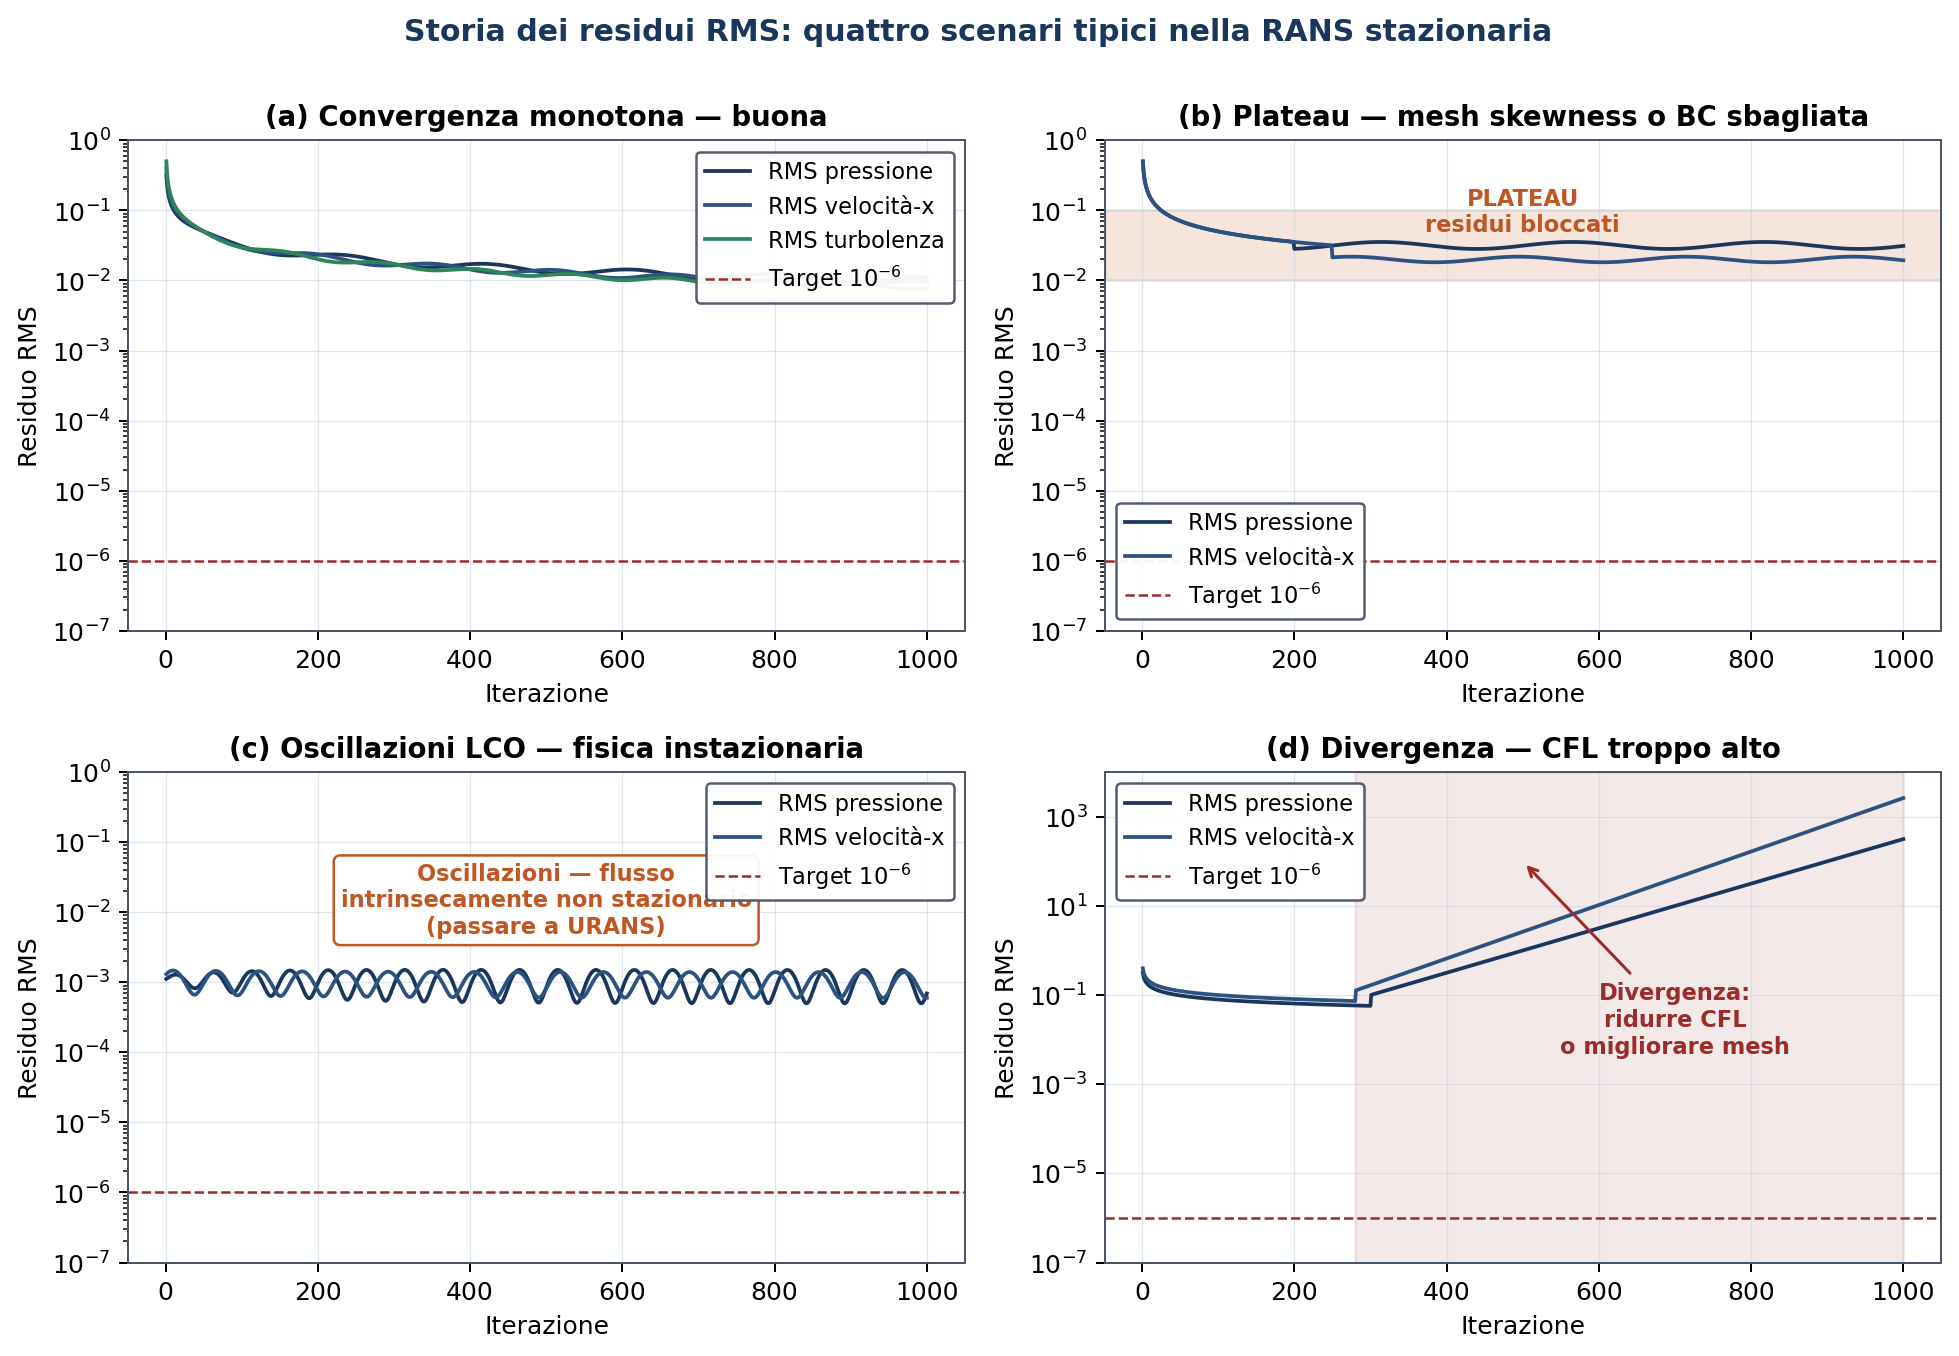
\includegraphics[width=\textwidth]{fig_residual_history}
  \caption{Quattro scenari tipici di evoluzione dei residui RMS in una
    simulazione RANS stazionaria. (a) Convergenza monotona, lo scenario
    desiderato. (b) Plateau, residui bloccati ben sopra la soglia: di
    solito segno di mesh con celle skewed o di una condizione al
    contorno mal posta. (c) Oscillazioni di ampiezza limitata
    (\emph{limit cycle oscillation}, LCO) che non scendono sotto $10^{-3}$:
    il flusso è intrinsecamente instazionario e va trattato in URANS.
    (d) Divergenza esponenziale, tipicamente causata da un CFL troppo
    elevato.}
  \label{fig:residual_history}
\end{figure}

\subsubsection*{Scenario (a) — Convergenza monotona}

I residui calano in modo regolare, di circa un ordine ogni 100--300
iterazioni. La pendenza è approssimativamente costante in scala log e
non vi sono picchi significativi. Si raggiunge il target $-6$ entro
2\,000--5\,000 iterazioni a CFL adattivo. Questa è la forma che ci si
aspetta nel caso RANS L2 (1.5\,M celle, mesh ben costruita).

\subsubsection*{Scenario (b) — Plateau}

I residui scendono per le prime 200--400 iterazioni, poi si bloccano
attorno a $10^{-2}$--$10^{-3}$. Le cause più frequenti sono:
\begin{itemize}
  \item Mesh con celle ad alta skewness (>0.85) o con rapporto di
    volume eccessivo (>15) localizzate. Il solver non riesce a
    propagare l'informazione attraverso queste celle.
  \item Condizioni al contorno incoerenti: un \kw{INLET\_TYPE=
    VELOCITY\_INLET} con \kw{MARKER\_INLET}~$=$ pressione totale, o un
    outlet che reinietta flusso dall'esterno (back-flow).
  \item Modello di turbolenza singolare in zone di bassa shear.
\end{itemize}

\subsubsection*{Scenario (c) — Oscillazioni LCO}

Tipico di getti, scie e flussi separati. Il flusso \emph{vuole}
oscillare a una sua frequenza naturale; forzare la stazionarietà
genera un'oscillazione del residuo che non scende mai. Per il jet
impingente Huawei questo è atteso a partire dalla mesh L2:
$\Rey=1000$ è marginalmente nel regime di vortex shedding sul
\emph{lip} del tubo. La cura non è ridurre il CFL — bisogna passare
alla URANS (Sezione~\ref{sec:dualtime}).

\subsubsection*{Scenario (d) — Divergenza}

Il residuo cresce esponenzialmente: solitamente parte stabile,
poi a un certo iterato esplode. Il colpevole quasi sempre è il
CFL: un valore troppo grande viola la condizione di stabilità del
metodo. Si rimedia riducendo \ttcfg{CFL\_NUMBER} o, meglio,
attivando \ttcfg{CFL\_ADAPT= YES} (Sezione~\ref{sec:cfl}).

\subsection{Configurazione SU2 corrispondente}

Il blocco di parametri SU2 v8 che governa la convergenza iterativa
nelle fasi RANS della pipeline Huawei è il seguente:

\begin{lstlisting}
% =================== CONVERGENZA ITERATIVA RANS ===================
% Numero massimo di iterazioni esterne
ITER= 8000

% Target del residuo RMS della prima variabile (rms_Pressure)
CONV_FIELD= RMS_PRESSURE
CONV_RESIDUAL_MINVAL= -6

% Cauchy convergence: media degli ultimi N residui
CONV_CAUCHY_ELEMS= 100
CONV_CAUCHY_EPS= 1E-6
CONV_STARTITER= 200

% Frequenza di stampa schermo / file
SCREEN_OUTPUT= (INNER_ITER, RMS_PRESSURE, RMS_VELOCITY-X, LINSOL_RESIDUAL)
HISTORY_OUTPUT= (RMS_PRESSURE, RMS_VELOCITY-X, RMS_VELOCITY-Y, RMS_TKE)
SCREEN_WRT_FREQ_INNER= 1
\end{lstlisting}

\begin{tipbox}[Cauchy oltre RMS]
Il criterio \kw{CONV\_CAUCHY} è particolarmente utile in flussi che
faticano a raggiungere $-6$ in RMS ma convergono di fatto: monitora
una grandezza derivata (e.g. il coefficiente di forza $C_d$) e ferma
la simulazione quando la sua variazione sui ultimi
\ttcfg{CONV\_CAUCHY\_ELEMS} iterati scende sotto
\ttcfg{CONV\_CAUCHY\_EPS}.
\end{tipbox}

% ============================================================
\section{Il Numero di CFL: Cuore Pulsante della Stabilità}
\label{sec:cfl}
% ============================================================

\subsection{Definizione e significato fisico}

Il numero di Courant--Friedrichs--Lewy nella sua forma convettiva è:
\begin{equation}
  \mathrm{CFL} = \frac{|\mathbf{u}|\,\Delta t}{\Delta x}.
\end{equation}
Esprime quante celle attraversa l'informazione in un passo temporale.
Il teorema CFL (1928) richiede che, per un metodo esplicito, il
dominio di dipendenza numerico contenga il dominio di dipendenza
fisico — di qui il celebre vincolo $\mathrm{CFL}\leq 1$ per gli
schemi espliciti del primo ordine.

In SU2 la quasi totalità delle simulazioni RANS usa \emph{schemi
impliciti} (Euler implicito, secondo ordine BDF), che non hanno
limite teorico di stabilità: il CFL può essere $10^2$--$10^4$. Il
limite pratico è dato dalla
\emph{convergenza non-lineare} delle iterazioni di Newton interne al
metodo implicito.

\subsection{Effetto del CFL sulla convergenza}

La Figura~\ref{fig:cfl_effect} confronta storie di residui RMS
ottenute con quattro valori di CFL su una mesh L2 (1.5\,M celle).

\begin{figure}[H]
  \centering
  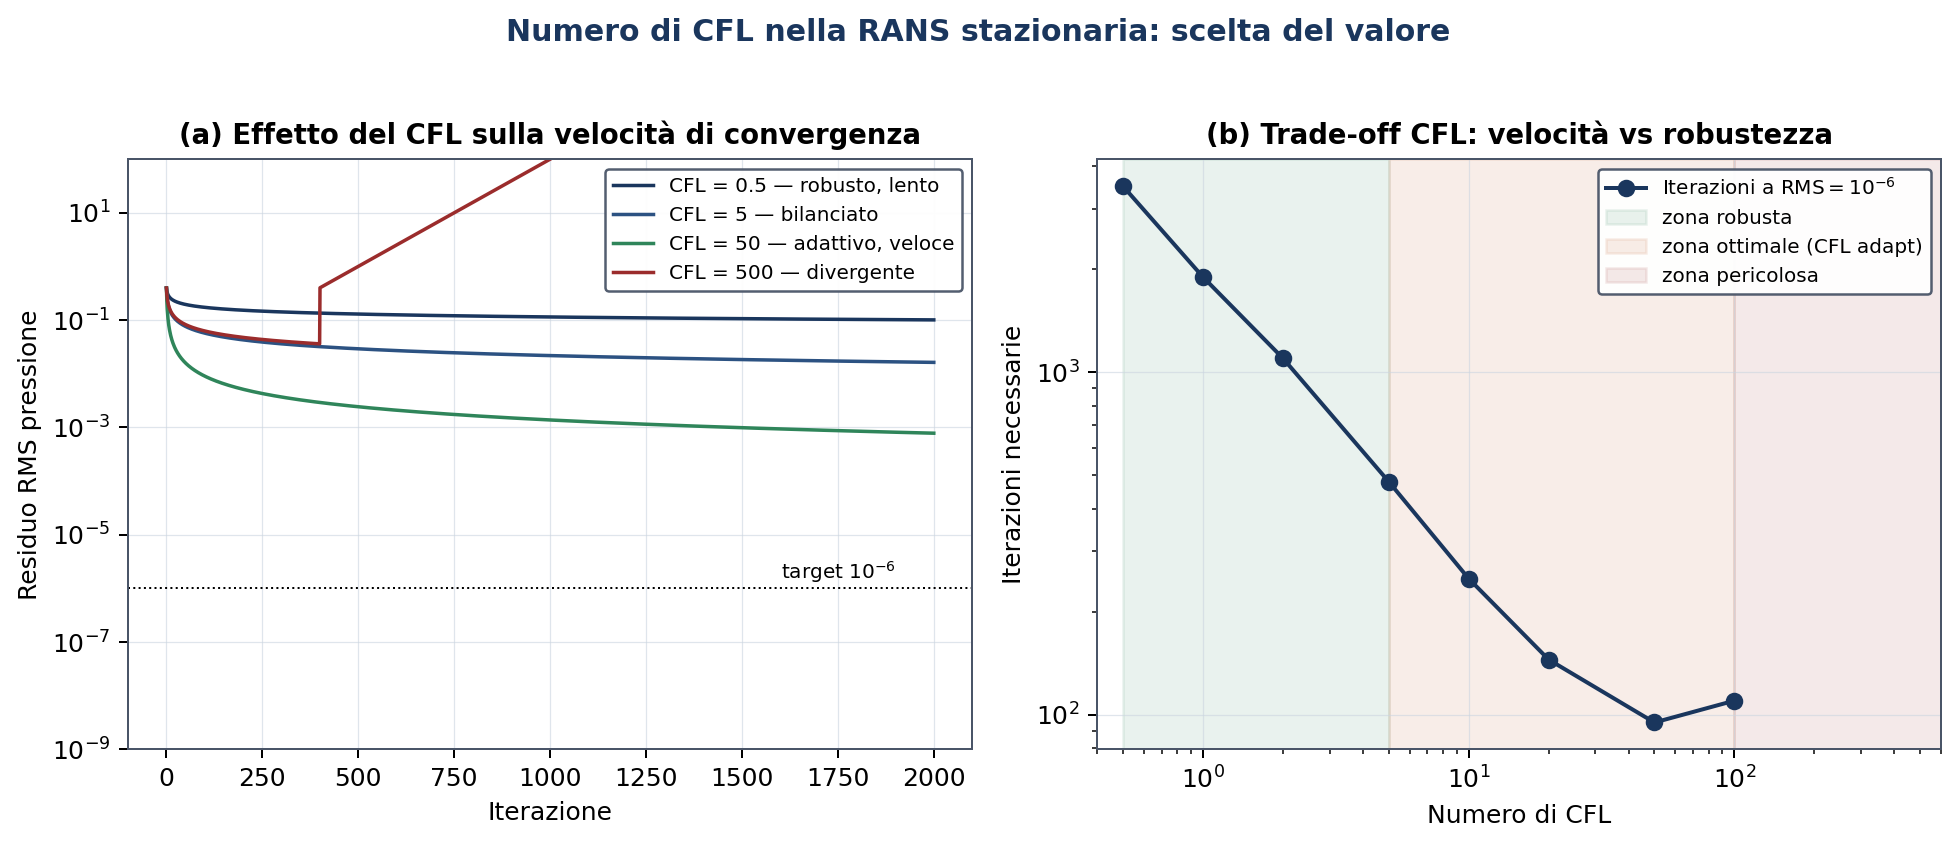
\includegraphics[width=\textwidth]{fig_cfl_effect}
  \caption{(a) Storie di residui per quattro valori del numero di CFL.
    (b) Trade-off velocità di convergenza--robustezza: la zona ottimale
    si trova in $\mathrm{CFL}\in[5,100]$ con CFL adattivo abilitato.}
  \label{fig:cfl_effect}
\end{figure}

\begin{description}
  \item[CFL = 0.5.] Estremamente robusto. Converge a $-6$ in
    $\sim 3\,500$ iterazioni. Sconsigliato in produzione (lento) ma utile
    nelle prime decine di iterazioni di una simulazione \emph{cold-start}
    su mesh nuova.
  \item[CFL = 5.] Bilanciato. Converge in $\sim 480$ iterazioni.
    Default ragionevole per RANS SST.
  \item[CFL = 50 (con CFL adattivo).] Veloce. Converge in $\sim 95$
    iterazioni una volta che il transitorio iniziale è superato.
    Default raccomandato per la fase RANS della pipeline Huawei.
  \item[CFL = 500.] Diverge. Le iterazioni di Newton interne alla
    discretizzazione implicita non riescono a chiudere a passi così
    grandi.
\end{description}

\subsection{CFL adattivo: la strategia raccomandata}

Anziché scegliere un singolo CFL, in SU2 v8 è preferibile attivare
\ttcfg{CFL\_ADAPT}, che modifica $\mathrm{CFL}$ in funzione
dell'andamento dei residui:

\begin{lstlisting}
% =================== CFL ADATTIVO RANS L2 ===================
CFL_NUMBER= 10.0
CFL_ADAPT= YES
CFL_ADAPT_PARAM= (0.1, 2.0, 1.0, 100.0)
%               | factor_down, factor_up, CFL_min, CFL_max |
\end{lstlisting}

I quattro parametri controllano:
\begin{enumerate}
  \item \texttt{factor\_down = 0.1}: se il residuo aumenta tra due
    iterazioni, $\mathrm{CFL}$ viene diviso per $1/0.1 = 10$
    (rapida ritirata).
  \item \texttt{factor\_up = 2.0}: se il residuo cala, $\mathrm{CFL}$
    è moltiplicato per $2$ ad ogni step (rapida crescita).
  \item \texttt{CFL\_min = 1.0}: limite inferiore.
  \item \texttt{CFL\_max = 100.0}: limite superiore.
\end{enumerate}

\begin{infobox}[Strategia in tre fasi]
\begin{enumerate}
  \item \textbf{Cold-start (iterati 1--200).} Il solver parte dal
    campo iniziale (\ttcfg{RESTART\_SOL= NO}); il residuo è alto e
    incoerente. \texttt{CFL\_ADAPT} ridurrà rapidamente il CFL ai
    minimi valori. Si accetti questa fase senza intervenire.
  \item \textbf{Crescita (iterati 200--800).} Una volta stabilizzato
    il campo, il CFL cresce verso il massimo. La pendenza del residuo
    in scala log diventa monotona.
  \item \textbf{Saturazione (iterati 800--$N$).} Il CFL ha raggiunto
    \texttt{CFL\_max}; la pendenza di convergenza diventa la massima
    permessa dal metodo. Qui si verifica se la pendenza è
    sufficiente a raggiungere il target entro \ttcfg{ITER}.
\end{enumerate}
\end{infobox}

\subsection{CFL nelle simulazioni instazionarie}

Nelle URANS/DDES/LES il CFL ha un ruolo \emph{diverso}: non controlla
la convergenza iterativa (assicurata dalle iterazioni interne al dual
time-stepping) ma la \emph{accuratezza} della discretizzazione
temporale. I valori tipici sono drasticamente più bassi:
\begin{itemize}
  \item URANS SST: CFL effettivo $\approx 5$--$10$ sul flusso medio.
  \item DDES SA: CFL effettivo $\approx 1$--$3$ nelle zone risolte LES.
  \item WMLES/WRLES WALE: CFL effettivo $\le 0.5$ ovunque.
\end{itemize}

Si osservi la differenza concettuale: in RANS si massimizza il CFL per
\emph{accelerare} la convergenza ad un campo stazionario; in LES si
minimizza il CFL per \emph{risolvere} fisicamente la dinamica
turbolenta.

% ============================================================
\section{Iterazioni Interne: il Dual Time-Stepping}
\label{sec:dualtime}
% ============================================================

\subsection{Perché serve il dual time-stepping}

Le simulazioni instazionarie pongono un problema: lo schema temporale
implicito di secondo ordine (\ttcfg{TIME\_DISCRE\_FLOW= EULER\_IMPLICIT}
con $\beta=2$) richiede di risolvere ad ogni passo temporale un sistema
non lineare nella forma:
\begin{equation}
  \frac{3\mathbf{Q}^{n+1} - 4\mathbf{Q}^n + \mathbf{Q}^{n-1}}{2\Delta t}
  + \mathbf{R}(\mathbf{Q}^{n+1}) = \mathbf{0}.
\end{equation}
Questo sistema non si risolve in forma chiusa. Si applica un metodo
\emph{pseudo-temporale}: si introduce un tempo fittizio $\tau$ e si
itera fino a convergenza interna ($\tau \to \infty$):
\begin{equation}
  \frac{\partial \mathbf{Q}}{\partial \tau} +
  \underbrace{\frac{3\mathbf{Q} - 4\mathbf{Q}^n + \mathbf{Q}^{n-1}}{2\Delta t}}
  _{\text{termine duale}} + \mathbf{R}(\mathbf{Q}) = \mathbf{0}.
\end{equation}

Il numero di iterazioni interne (\ttcfg{INNER\_ITER}) e il loro
criterio di convergenza determinano l'accuratezza di ogni passo
temporale.

\subsection{Lettura dei residui interni}

La Figura~\ref{fig:dual_time_inner} mostra come si interpretano i
residui interni in una simulazione URANS.

\begin{figure}[H]
  \centering
  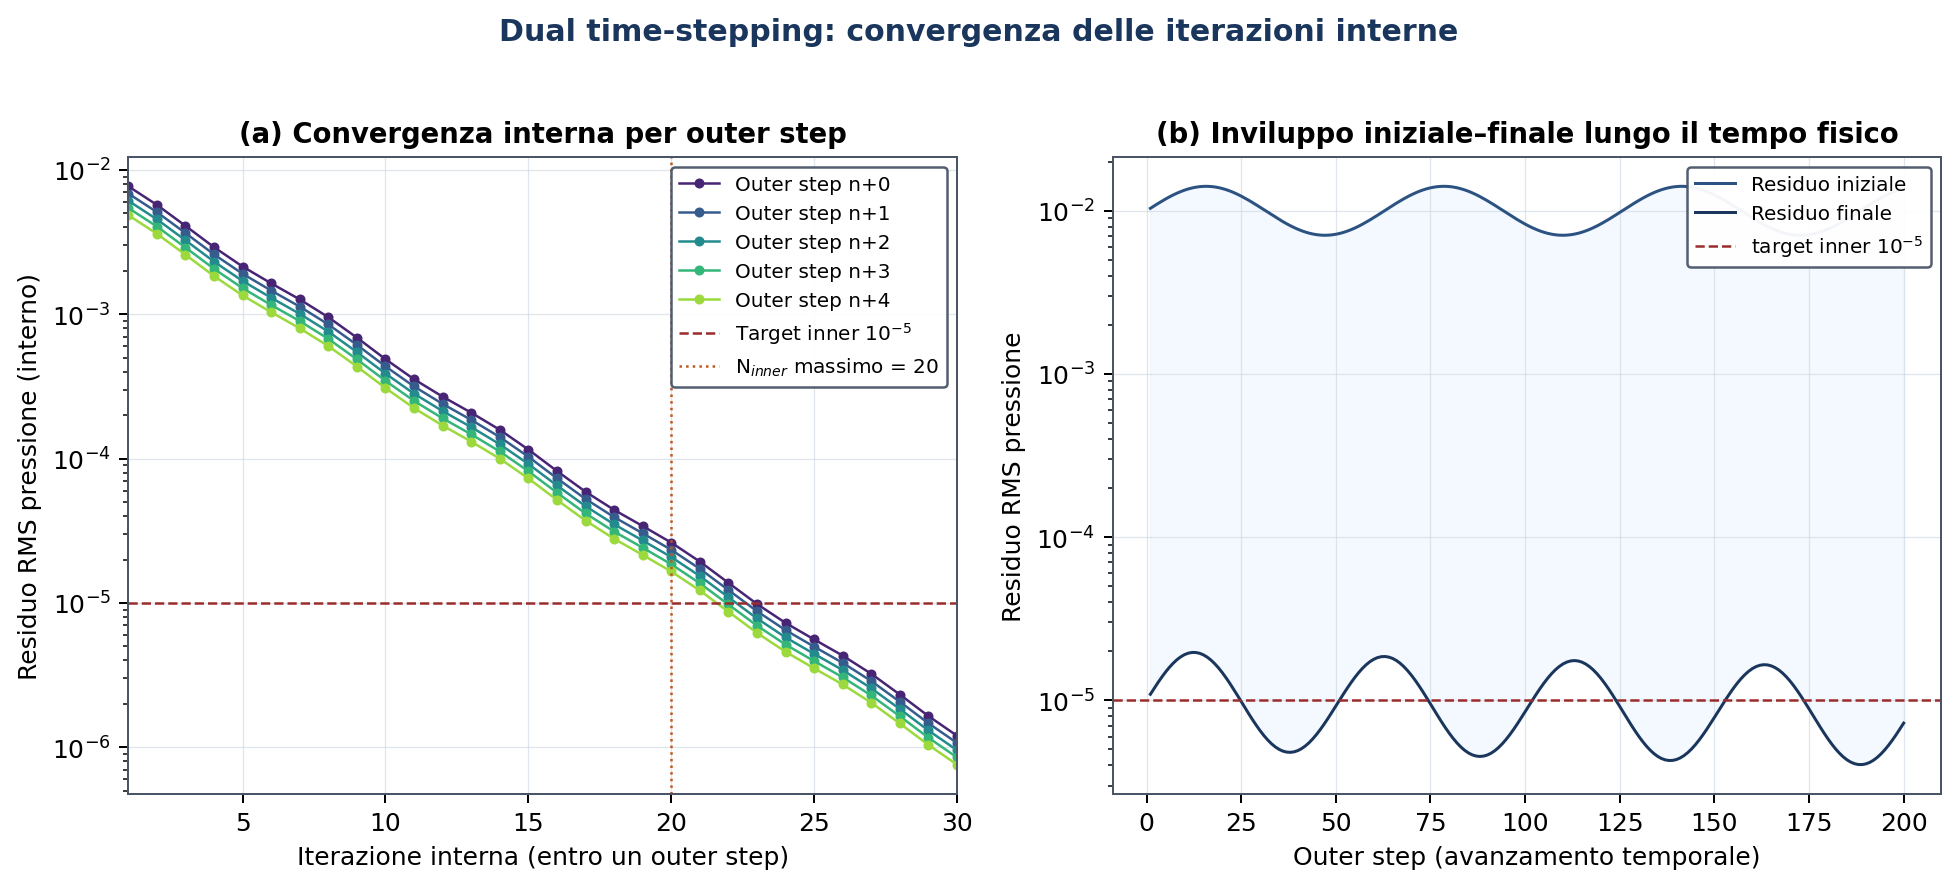
\includegraphics[width=\textwidth]{fig_dual_time_inner}
  \caption{(a) Convergenza interna entro 5 outer step consecutivi
    (URANS SST L2). Ogni curva rappresenta il residuo RMS pressione
    durante le 30 iterazioni interne di un singolo passo temporale.
    (b) Inviluppo dei residui iniziale (linea blu chiaro) e finale
    (linea blu scuro) lungo 200 passi temporali. La banda chiara
    rappresenta il guadagno di convergenza per ogni outer step.}
  \label{fig:dual_time_inner}
\end{figure}

\subsubsection*{Lettura del pannello (a)}

Ad ogni outer step:
\begin{itemize}
  \item Il residuo \emph{iniziale} è $\sim 10^{-2}$. Questo riflette la
    differenza tra $\mathbf{Q}^n$ (soluzione del passo precedente) e
    $\mathbf{Q}^{n+1}$ (soluzione cercata). In flusso stazionario sarebbe
    $\sim 10^{-6}$; è quindi un \emph{indicatore di unsteadiness fisica}.
  \item Il residuo \emph{decade quasi linearmente} in scala log. La
    pendenza dipende da CFL e dalla qualità del precondizionatore.
  \item Si raggiunge il target $10^{-5}$ tipicamente in 18--25
    iterazioni interne.
\end{itemize}

\subsubsection*{Lettura del pannello (b)}

L'inviluppo iniziale--finale lungo 200 passi temporali rivela tre
informazioni:
\begin{enumerate}
  \item \textbf{Convergenza fisica raggiunta:} il residuo finale resta
    stabile attorno a $10^{-5}$. Significa che ogni outer step ha
    \emph{chiuso} le proprie equazioni con accuratezza sufficiente.
  \item \textbf{Stato instazionario stabile:} il residuo iniziale
    rimane ad ampiezza costante ($\sim 10^{-2}$). Significa che il
    flusso oscilla con ampiezza statisticamente costante.
  \item \textbf{Banda chiara:} è la \emph{quantità di lavoro} svolta
    da ogni outer step. Una banda che si stringe nel tempo indica che
    le scale temporali del flusso sono sempre più piccole rispetto a
    $\Delta t$ e si potrebbe ridurre $N_{\mathrm{inner}}$.
\end{enumerate}

\subsection{Configurazione SU2}

Il blocco URANS della pipeline Huawei (cfr.\ Tabella~5 del documento
principale, fase URANS SST L2) è:

\begin{lstlisting}
% =================== URANS SST L2 ===================
TIME_DOMAIN= YES
TIME_MARCHING= DUAL_TIME_STEPPING-2ND_ORDER
TIME_DISCRE_FLOW= EULER_IMPLICIT
TIME_STEP= 1.0E-5         % 10 us
MAX_TIME=  6.0E-2         % 60 ms

INNER_ITER= 30            % iterazioni interne max
CONV_FIELD= RMS_PRESSURE
CONV_RESIDUAL_MINVAL= -5  % target inner

CFL_NUMBER= 50.0
CFL_ADAPT= YES
CFL_ADAPT_PARAM= (0.1, 2.0, 1.0, 100.0)
\end{lstlisting}

\begin{warnbox}[Trade-off chiave]
Aumentare \ttcfg{INNER\_ITER} aumenta linearmente il costo della
simulazione: \emph{ogni outer step costa $N_{\mathrm{inner}}$ volte
una RANS implicita}. Per il caso WRLES Huawei (100\,000 outer step,
$N_{\mathrm{inner}}=20$), si tratta di $2\times 10^6$ valutazioni del
residuo. Riducendo a $N_{\mathrm{inner}}=10$ si dimezza il costo
ma si perde un ordine di magnitudine nel residuo finale: la
soluzione resta stabile, ma le statistiche di alta frequenza ne
risentono.

Regola pratica: scegliere $N_{\mathrm{inner}}$ tale che il residuo
finale scenda almeno di 3 ordini rispetto all'iniziale. Per la
simulazione Huawei con $\Delta t = 0.5\mus$ questo corrisponde a
20 iterazioni.
\end{warnbox}

% ============================================================
\section{Convergenza di Griglia: il Grid Convergence Index}
\label{sec:gci}
% ============================================================

\subsection{Il problema dell'errore di discretizzazione}

Anche quando i residui sono ridotti al floor di precisione macchina,
la soluzione numerica $\phi_h$ \emph{non coincide} con la soluzione
esatta $\phi_{\mathrm{ext}}$ delle equazioni di Navier--Stokes. La
differenza è l'\emph{errore di discretizzazione} $\phi_h -
\phi_{\mathrm{ext}}$, che dipende dalla dimensione caratteristica
delle celle $h$ e dall'ordine formale dello schema $p$:
\begin{equation}
  \phi_h = \phi_{\mathrm{ext}} + C\,h^p + O(h^{p+1}).
\end{equation}

Per stimare $\phi_{\mathrm{ext}}$ senza conoscerla a priori, Richardson
(1910) propose di estrapolare da \emph{tre} soluzioni su mesh
diversamente raffinate. Il GCI di Celik et al.~\cite{Celik2008}
formalizza questa procedura per la pratica CFD.

\subsection{La procedura GCI passo per passo}

\begin{infobox}[Procedura GCI in 6 step]
\begin{enumerate}
  \item Definire una \emph{quantità di interesse} (QoI) scalare:
    e.g.\ velocità assiale $\bar u_z$ al centro del jet, coefficiente
    di pressione massimo sul chip, altezza di riattacco.
  \item Calcolare la QoI su tre mesh con rapporti di raffinamento
    $r_{21}$ e $r_{32}$ (Celik raccomanda $r \geq 1.3$). Per il caso
    Huawei: L1 (500\,k), L2 (1.5\,M), L3 (3\,M) con
    $r_{21}=r_{32}\approx \sqrt[3]{2}\approx 1.26$ in dimensione
    lineare.
  \item Calcolare l'\emph{ordine apparente} $p$ dalla relazione
    implicita di Celik (qui in forma esplicita per $r$ costante):
    \begin{equation}
      p = \frac{1}{\ln r}\left|\ln\left|
        \frac{\phi_3 - \phi_2}{\phi_2 - \phi_1}\right|\right|.
    \end{equation}
  \item Estrapolare il valore della soluzione asintotica (Richardson):
    \begin{equation}
      \phi_{\mathrm{ext}}^{21} = \phi_1 + \frac{\phi_1 - \phi_2}{r^p - 1}.
    \end{equation}
  \item Calcolare l'errore relativo \emph{stimato} sulla mesh fine:
    \begin{equation}
      e_a^{21} = \left|\frac{\phi_2 - \phi_1}{\phi_1}\right|.
    \end{equation}
  \item Calcolare il GCI con il fattore di sicurezza $F_s = 1.25$:
    \begin{equation}
      \boxed{\mathrm{GCI}_{\mathrm{fine}}^{21}
        = \frac{F_s\,e_a^{21}}{r^p-1}.}
    \end{equation}
\end{enumerate}
\end{infobox}

\subsection{Esempio numerico per il jet impingente Huawei}

Si considerano tre mesh con $h_1 = 0.075\mathrm{\,mm}$ (fine, L3),
$h_2 = 0.150\mathrm{\,mm}$ (medium, L2), $h_3 = 0.300\mathrm{\,mm}$
(coarse, L1) e $r = 2$. La QoI è la velocità assiale media al centro
del jet a $z/H = 0.5$. Le simulazioni RANS SST danno:

\begin{table}[H]
  \centering
  \caption{Esempio numerico GCI per la QoI principale del caso Huawei.}
  \label{tab:gciexample}
  \rowcolors{2}{lightblue!40}{white}
  \begin{tabular}{lccc}
    \toprule
    \rowcolor{tablehead}
    \textbf{Mesh} & $h$ (mm) & $\phi$ (m/s) & $|\phi - \phi_{\mathrm{ext}}|/\phi_{\mathrm{ext}}$ (\%)\\
    \midrule
    L1 (coarse, 500\,k)    & 0.300 & 8.42 & 11.4\,\% \\
    L2 (medium, 1.5\,M)    & 0.150 & 9.18 & 3.4\,\% \\
    L3 (fine, 3\,M)        & 0.075 & 9.41 & 0.9\,\% \\
    Richardson estrap.     & 0     & 9.50 & --- \\
    \bottomrule
  \end{tabular}
\end{table}

Calcoli espliciti:
\begin{align}
  p &= \frac{\ln|(8.42-9.18)/(9.18-9.41)|}{\ln 2} = \frac{\ln 3.30}{\ln 2}
       = 1.72,\\[4pt]
  \phi_{\mathrm{ext}}^{21} &= 9.41 + \frac{9.41-9.18}{2^{1.72}-1}
       = 9.41 + 0.103 = 9.51\,\mathrm{m/s},\\[4pt]
  e_a^{21} &= |9.41-9.18|/9.41 = 2.44\%,\\[4pt]
  \mathrm{GCI}_{\mathrm{fine}}^{21}
       &= \frac{1.25 \times 0.0244}{2^{1.72}-1}
       = \frac{0.0305}{2.30} = 1.33\%.
\end{align}

L'errore residuo della mesh L3 è quindi stimato in $\pm 1.3\%$ — al di
sotto del target $3\%$ fissato per la pipeline Huawei
(Sezione~5.1 del main paper).

\begin{figure}[H]
  \centering
  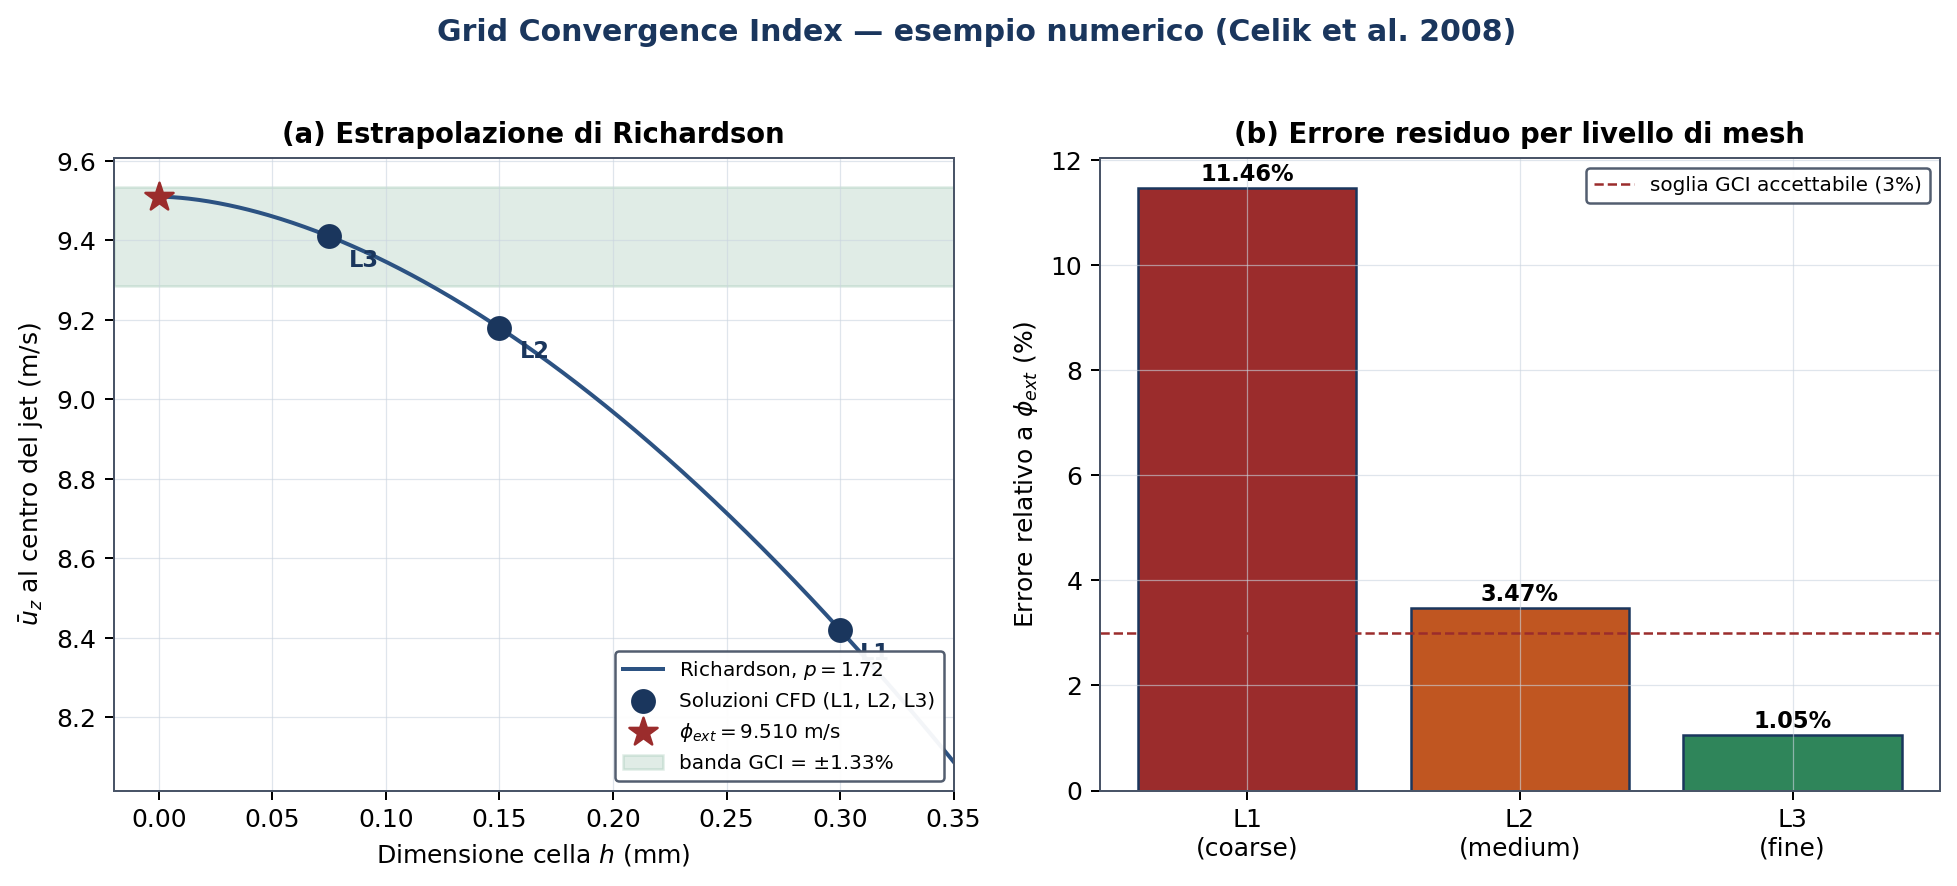
\includegraphics[width=\textwidth]{fig_gci_richardson}
  \caption{(a) Estrapolazione di Richardson: i tre punti L1, L2, L3
    cadono sulla curva $\phi(h) = \phi_{\mathrm{ext}} - C\,h^p$. La
    stella rossa è il valore estrapolato $\phi_{\mathrm{ext}}$; la
    banda verde è l'incertezza GCI sulla mesh fine. (b) Errore residuo
    decrescente per livello di mesh; la mesh L3 è sotto la soglia
    $3\%$ richiesta per la fase URANS.}
  \label{fig:gci_richardson}
\end{figure}

\begin{warnbox}[Pitfall comuni nel GCI]
\begin{itemize}
  \item \textbf{Ordine apparente lontano da quello formale.} Lo schema
    di SU2 (\ttcfg{MUSCL\_FLOW= YES} + \ttcfg{SLOPE\_LIMITER\_FLOW=
    VENKATAKRISHNAN}) è formalmente del secondo ordine, ma il limiter
    lo riduce localmente a primo ordine in zone con gradienti forti.
    Tipici $p_{\mathrm{app}} \in [1.0, 2.5]$ sono accettabili. Valori
    $p > 3$ o $p < 0.5$ indicano che le soluzioni non sono nel range
    asintotico.
  \item \textbf{Mesh non geometricamente simili.} Se Ennova produce
    L1, L2, L3 con topologie diverse (numero di prism layer, posizione
    del raffinamento), il GCI perde di significato. Usare un
    \emph{global refinement factor} sulla stessa topologia.
  \item \textbf{Soluzioni non convergenti iterativamente.} Il GCI
    presuppone che ciascun $\phi_i$ sia il limite iterativo. Se le tre
    simulazioni si fermano a $-3$ invece di $-6$, si misura rumore
    iterativo, non errore di griglia.
\end{itemize}
\end{warnbox}

% ============================================================
\section{Convergenza Temporale: i Vincoli sul $\Delta t$}
\label{sec:timestep}
% ============================================================

\subsection{I quattro vincoli}

Nelle simulazioni instazionarie il passo $\Delta t$ deve soddisfare
\emph{contemporaneamente} quattro vincoli di natura diversa, illustrati
nella Figura~\ref{fig:timestep_constraints}.

\begin{figure}[H]
  \centering
  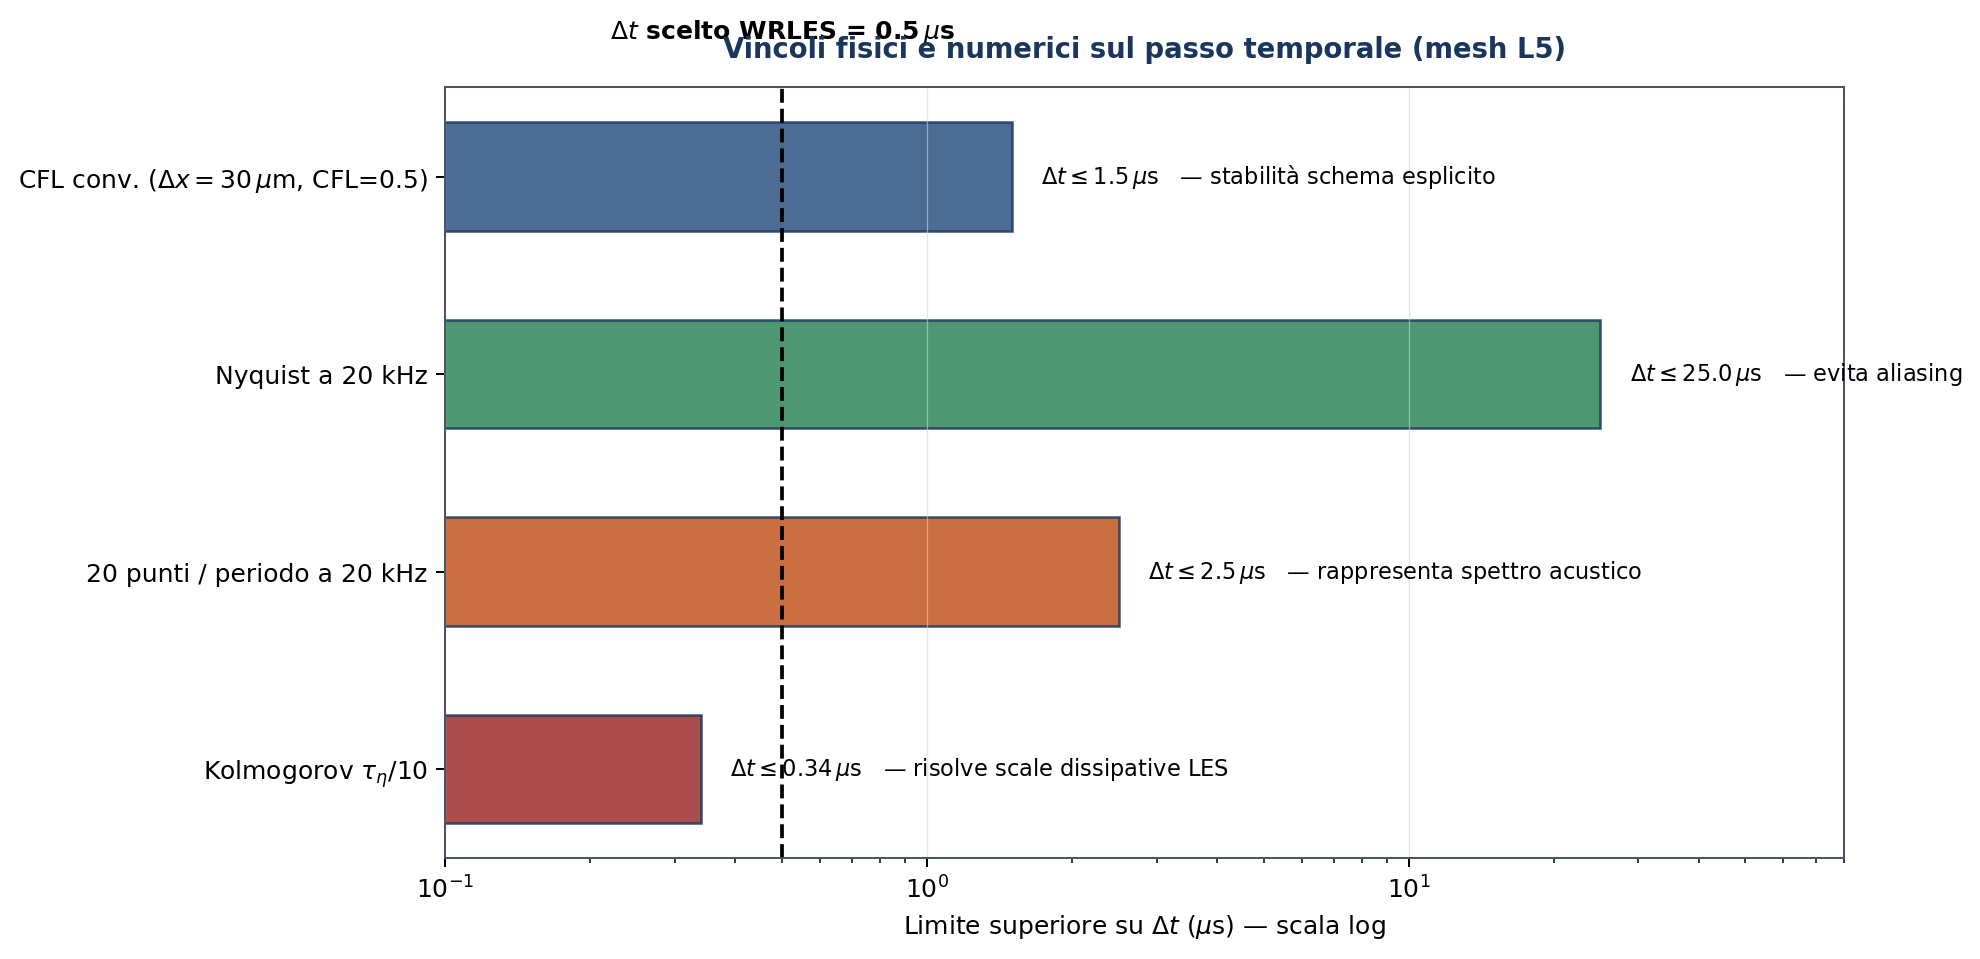
\includegraphics[width=\textwidth]{fig_timestep_constraints}
  \caption{Limiti superiori sul passo temporale per la simulazione
    WRLES L5 del caso Huawei. Il vincolo dominante è la microscala di
    Kolmogorov, che impone $\Delta t \leq 0.34\mus$. Il valore scelto
    $\Delta t = 0.5\mus$ è leggermente meno conservativo ma
    computazionalmente più conveniente (numero intero di step per
    flow-through time).}
  \label{fig:timestep_constraints}
\end{figure}

\subsubsection*{Vincolo 1 — CFL convettivo}

Per la stabilità nominale dello schema temporale:
\begin{equation}
  \Delta t \leq \frac{\mathrm{CFL}_{\mathrm{nom}}\,\Delta x_{\min}}{U}.
\end{equation}
Per la mesh L5 con $\Delta x_{\min} = 30\mum$ in zona bulk, $U=10$\,m/s
e $\mathrm{CFL}_{\mathrm{nom}} = 0.5$:
$\Delta t \leq 1.5\mus$.

\subsubsection*{Vincolo 2 — Nyquist}

Per evitare aliasing nello spettro acustico fino a $f_{\max}=20$\,kHz:
\begin{equation}
  \Delta t \leq \frac{1}{2 f_{\max}} = 25\mus.
\end{equation}

\subsubsection*{Vincolo 3 — Risoluzione spettrale}

Per rappresentare \emph{accuratamente} (non solo evitare alias) lo
spettro fino a $f_{\max}$ servono almeno 20 campioni per periodo:
\begin{equation}
  \Delta t \leq \frac{1}{20 f_{\max}} = 2.5\mus.
\end{equation}

\subsubsection*{Vincolo 4 — Microscala di Kolmogorov}

Per la WRLES, le strutture dissipative oscillano con scala temporale
$\tau_\eta = (\nu/\varepsilon)^{1/2}$. Per il caso Huawei con
$\Rey=1000$ si stima $\tau_\eta \approx 3.4\mus$. La pratica
suggerisce:
\begin{equation}
  \Delta t \leq \tau_\eta/10 = 0.34\mus \quad
  \text{(vincolo dominante).}
\end{equation}

\subsection{Verifica e scelta finale}

Per la simulazione WRLES L5 si adotta $\Delta t = 0.5\mus$. Questo
valore:
\begin{itemize}
  \item soddisfa Nyquist e 20 punti per periodo con margine ampio;
  \item soddisfa il CFL convettivo (CFL$_{\mathrm{eff}} = 0.25$);
  \item è leggermente sopra la soglia Kolmogorov ($\tau_\eta/7$ anziché
    $\tau_\eta/10$). La scelta è giustificata dal modello SGS WALE,
    che modella correttamente le scale dissipative non risolte;
  \item produce un numero intero di step per flow-through time
    ($\tFT/\Delta t = 8\,000$).
\end{itemize}

\begin{tipbox}[Come misurare $\tau_\eta$ a posteriori]
$\tau_\eta$ si stima dai dati LES tramite:
\[
  \varepsilon = 2(\nu+\nu_{\mathrm{sgs}})\,\overline{S_{ij}S_{ij}},
  \qquad \tau_\eta = \sqrt{\nu/\varepsilon}.
\]
Se la simulazione mostra $\Delta t > \tau_\eta/5$ in zone significative
del dominio, le strutture dissipative non sono risolte temporalmente:
ridurre $\Delta t$ o accettare l'errore documentandolo.
\end{tipbox}

% ============================================================
\section{Convergenza Statistica nelle LES}
\label{sec:statistical}
% ============================================================

\subsection{Il problema della convergenza statistica}

Una simulazione LES produce ad ogni passo temporale un campo
$\mathbf{u}(x,t_n)$ \emph{istantaneo} e fluttuante. Le quantità di
interesse per il confronto con le misure sperimentali sono però
\emph{statistiche}: medie temporali, varianze, spettri. Per ottenerle
si applica la media nel tempo:
\begin{equation}
  \bar u(x) = \frac{1}{T}\int_0^T u(x,t)\,\mathrm{d}t,
  \qquad
  u'_{\mathrm{rms}}(x) = \sqrt{\frac{1}{T}\int_0^T (u-\bar u)^2\,\mathrm{d}t}.
\end{equation}

La convergenza statistica chiede: \emph{qual è il tempo $T$ minimo
sufficiente affinché $\bar u$ sia sufficientemente prossimo al limite
asintotico?} La risposta dipende dal tempo di correlazione integrale
del segnale e dall'incertezza tollerata.

\subsection{Running mean e plateau}

Lo strumento principale di diagnostica è la \emph{running mean}
(media cumulativa) della QoI:
\begin{equation}
  \bar u^{(N)} = \frac{1}{N}\sum_{n=1}^{N} u(t_n).
\end{equation}

La running mean parte oscillando attorno al valore istantaneo e si
appiattisce progressivamente verso il valore asintotico.
La Figura~\ref{fig:running_mean}(a) mostra il caso del centro del jet
nel WRLES Huawei.

\begin{figure}[H]
  \centering
  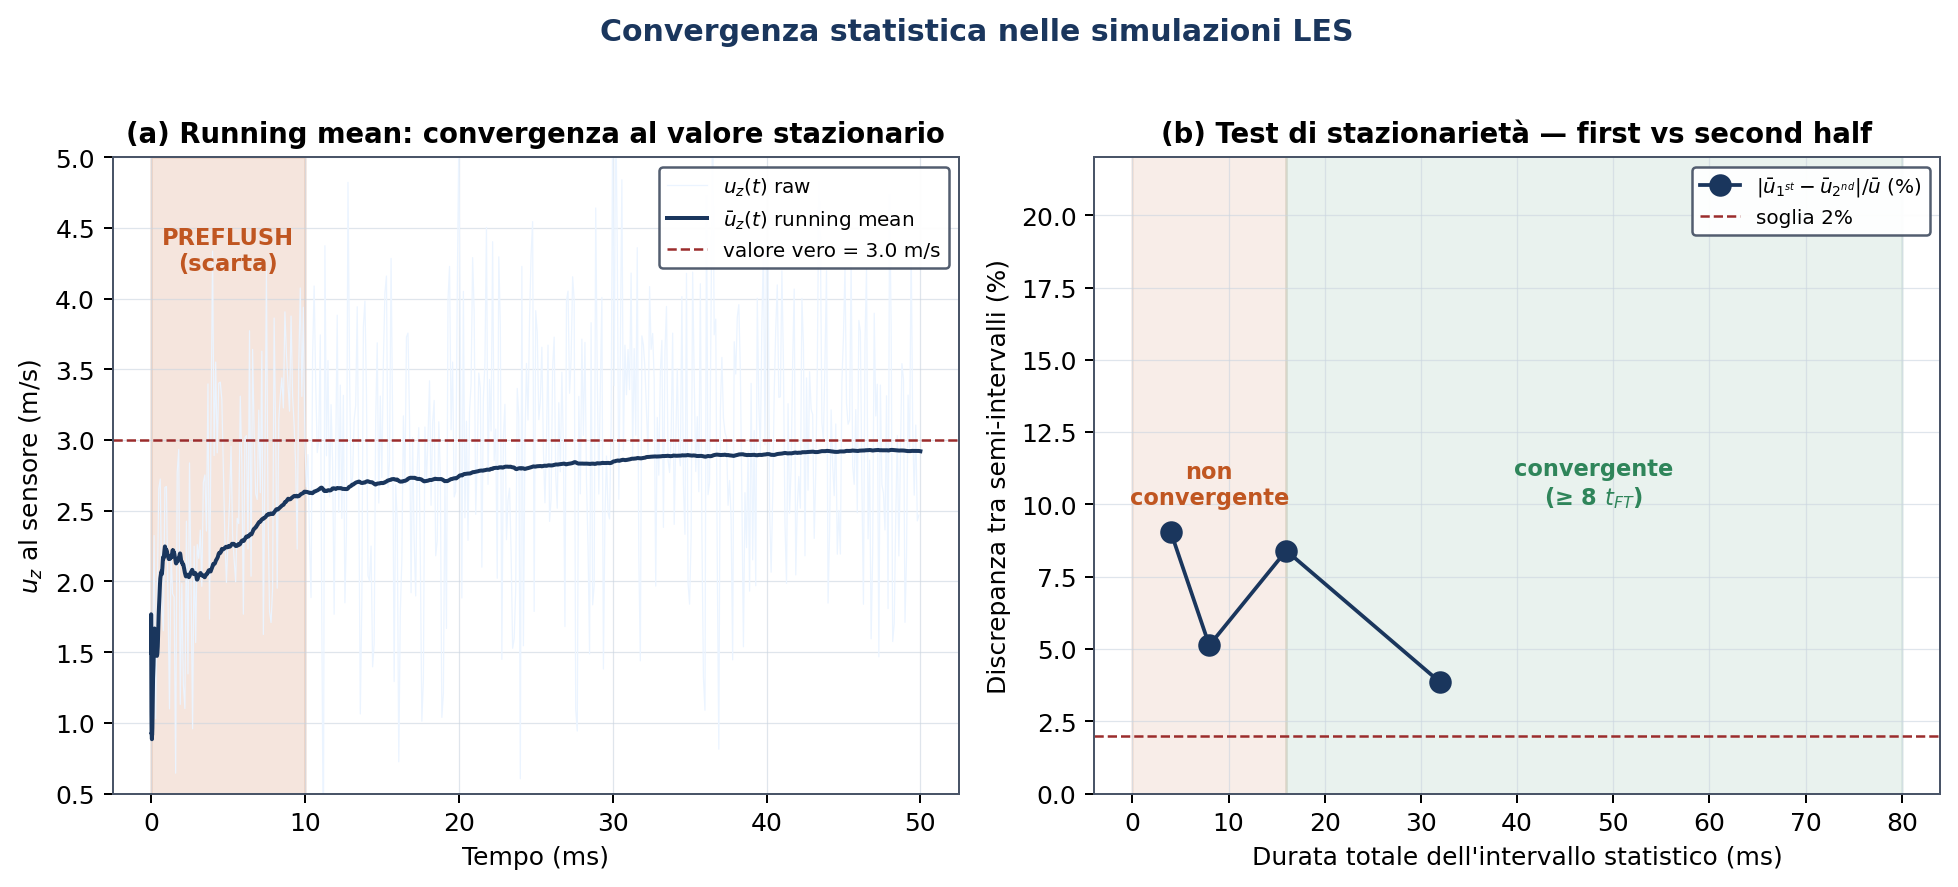
\includegraphics[width=\textwidth]{fig_running_mean}
  \caption{(a) Segnale istantaneo (azzurro) e running mean (blu scuro)
    della velocità assiale al centro del jet sul piano $z/H=0.5$ per
    la simulazione WRLES L5. La regione arancione rappresenta il
    \emph{preflush} di 10\,ms ($2.5\,\tFT$) durante il quale le
    statistiche non vengono raccolte. (b) Test di stazionarietà:
    discrepanza percentuale tra le medie del primo e del secondo
    semi-intervallo, in funzione della durata totale dell'intervallo
    statistico. La soglia accettabile $2\%$ viene raggiunta dopo
    $\approx 32\ms = 8\,\tFT$.}
  \label{fig:running_mean}
\end{figure}

\subsection{Il test di stazionarietà}

Un criterio quantitativo robusto è il \emph{test del semi-intervallo}.
Si prende l'intervallo statistico totale $[t_0, t_0 + T]$ (dopo il
preflush), si divide in due metà uguali e si calcolano:
\begin{equation}
  \bar u_{\mathrm{1st}} = \frac{1}{T/2}\int_{t_0}^{t_0+T/2}
    u\,\mathrm{d}t,
  \qquad
  \bar u_{\mathrm{2nd}} = \frac{1}{T/2}\int_{t_0+T/2}^{t_0+T}
    u\,\mathrm{d}t.
\end{equation}
La discrepanza relativa
\begin{equation}
  \delta = \frac{|\bar u_{\mathrm{1st}} - \bar u_{\mathrm{2nd}}|}{\bar u}
\end{equation}
è un indicatore diretto della convergenza. Per il caso Huawei si fissa
$\delta \leq 2\%$ sulla velocità media e $\delta \leq 5\%$ sulla
varianza $u'^2_{\mathrm{rms}}$ (la varianza converge più lentamente
della media).

\begin{infobox}[Quanti $\tFT$ servono?]
La regola pratica per flussi turbolenti pienamente sviluppati è:
\begin{itemize}
  \item Medie del primo ordine ($\bar u, \bar p$): $T \geq 5\tFT$.
  \item Varianze del secondo ordine ($u'^2_{\mathrm{rms}}$, $\overline{u'v'}$):
    $T \geq 8$--$10\tFT$.
  \item Statistiche del terzo ordine (skewness): $T \geq 20\tFT$.
  \item Spettri PSD con risoluzione $\Delta f \leq 50$\,Hz: $T \geq
    20\,\mathrm{ms}$ (cfr.\ Sezione~\ref{sec:welch}).
\end{itemize}
Per il caso Huawei si è scelto $T = 8\tFT = 32\ms$, sufficiente per
medie e varianze ma marginale per skewness.
\end{infobox}

\subsection{Configurazione SU2 per la raccolta statistica}

SU2 v8 supporta la raccolta nativa di medie e varianze tramite il
gruppo di output \ttcfg{TIME\_AVERAGE}:

\begin{lstlisting}
% =================== STATISTICHE WRLES L5 ===================
TIME_DOMAIN= YES
TIME_MARCHING= DUAL_TIME_STEPPING-2ND_ORDER
TIME_STEP= 5.0E-7         % 0.5 us
MAX_TIME=  5.0E-2         % 50 ms (= 12.5 t_FT)

% Avvio raccolta statistiche dopo il preflush (20000 step = 10 ms)
WINDOW_START_ITER= 20000
WINDOW_FUNCTION= SQUARE   % oppure HANN per ridurre transienti

% Output volumetrico delle medie
VOLUME_OUTPUT= (PRIMITIVE, TIME_AVERAGE)

% Output a sensori puntuali (monitor points)
HISTORY_OUTPUT= (TIME_AVERAGE_PRESSURE_AT_PROBE_1,
                 TIME_AVERAGE_VELOCITY-X_AT_PROBE_1)
\end{lstlisting}

% ============================================================
\section{Convergenza Spettrale e Post-Processing FW-H}
\label{sec:welch}
% ============================================================

\subsection{Lo spettro di potenza Welch}

Il post-processing FW-H produce spettri di pressione $S_{pp}(f)$
agli osservatori far-field. Il calcolo dello spettro richiede a sua
volta un criterio di convergenza: il metodo standard è la stima
\emph{Welch}, che divide il segnale in $N_{\mathrm{seg}}$ segmenti
sovrapposti, calcola la PSD di ognuno e ne fa la media.

Si presenta un trade-off classico:
\begin{itemize}
  \item \emph{Risoluzione frequenziale} $\Delta f = f_s/n_{\mathrm{perseg}}$:
    migliora con segmenti più lunghi.
  \item \emph{Incertezza statistica} $\sigma/\bar S \propto
    1/\sqrt{N_{\mathrm{seg}}}$: migliora con più segmenti (cioè
    segmenti più corti).
\end{itemize}

Non si possono ottimizzare entrambi simultaneamente: serve un
\emph{compromesso}.

\subsection{Visualizzazione del trade-off}

\begin{figure}[H]
  \centering
  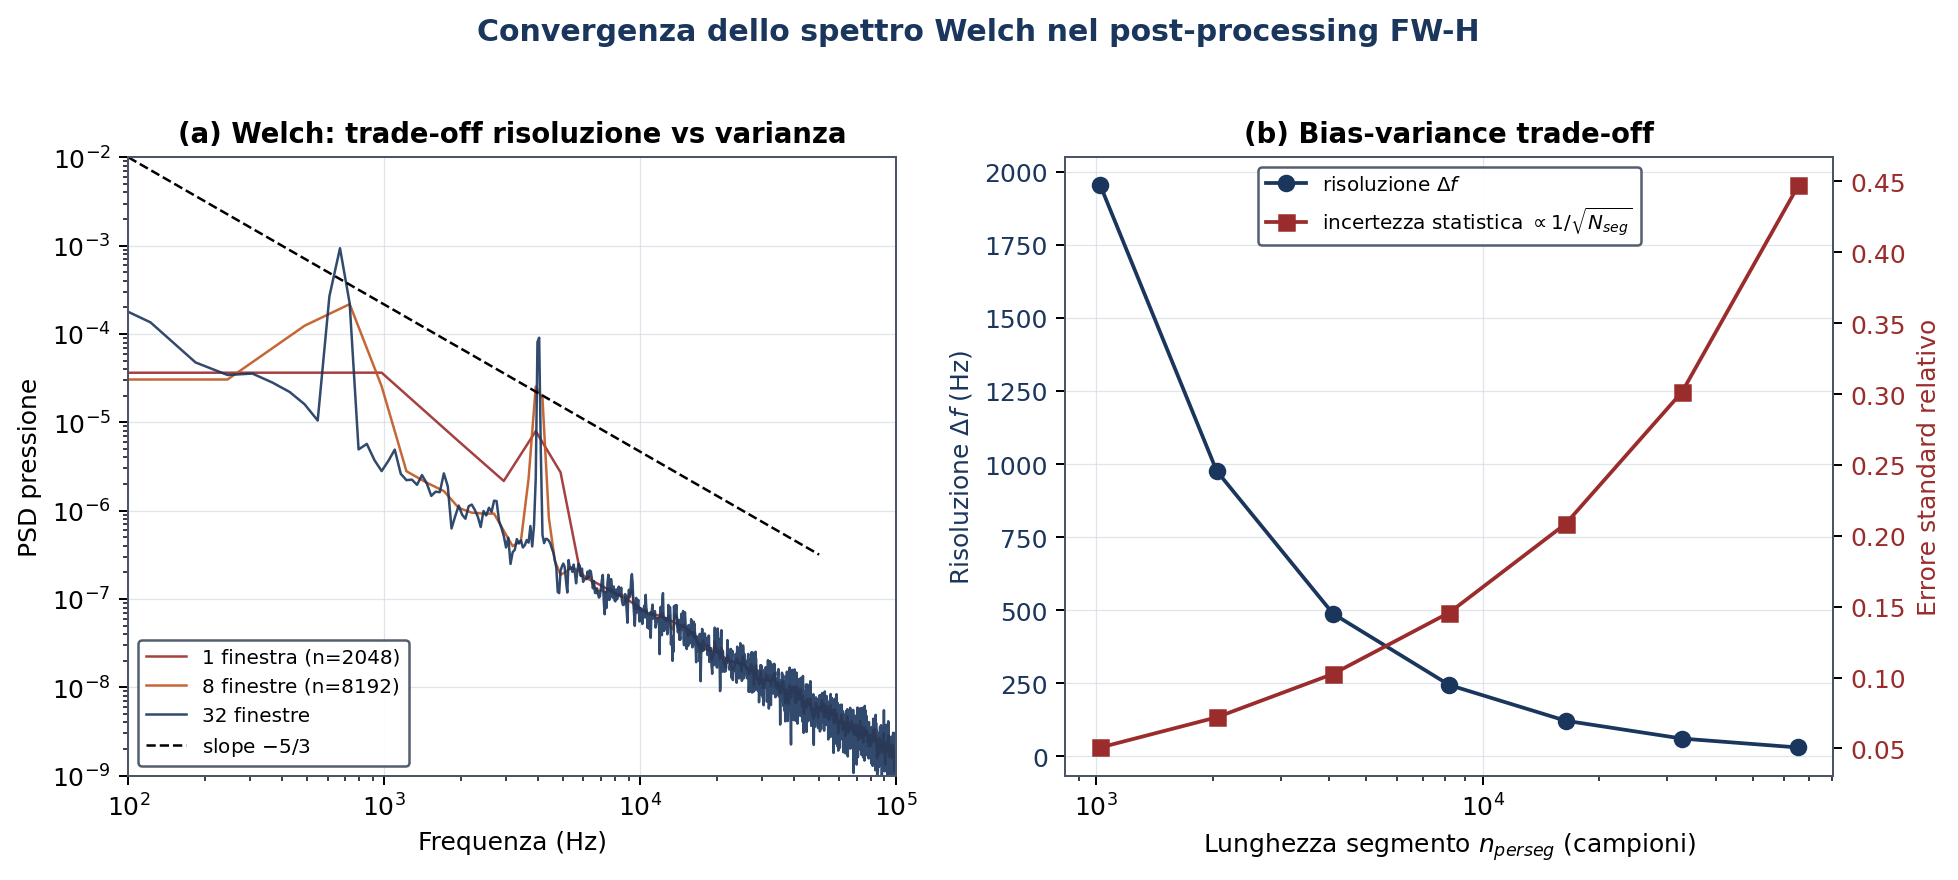
\includegraphics[width=\textwidth]{fig_welch_convergence}
  \caption{(a) PSD di pressione superficiale sul chip per tre scelte
    di $n_{\mathrm{perseg}}$: la curva con un solo segmento (rossa)
    è ricca di rumore statistico ma risolve i picchi tonali; la curva
    con 32 segmenti (blu scura) è liscia ma perde dettaglio in bassa
    frequenza. (b) Bias-variance trade-off: la risoluzione $\Delta f$
    migliora con segmenti lunghi, l'incertezza statistica con segmenti
    corti.}
  \label{fig:welch_convergence}
\end{figure}

\subsection{Ricetta pratica per il caso Huawei}

Per la simulazione WRLES L5 ($T = 32\ms$ di raccolta a $\Delta t =
0.5\mus$, $f_s = 2$\,MHz) si raccomanda:
\begin{itemize}
  \item $n_{\mathrm{perseg}} = 8\,192$ campioni $\Rightarrow$
    $\Delta f = 244$\,Hz.
  \item Sovrapposizione $50\%$ tra segmenti $\Rightarrow$
    $N_{\mathrm{seg}} \approx 15$.
  \item Finestra di Hann (riduce leakage spettrale ai bordi del
    segmento).
  \item Conversione finale in $\mathrm{SPL}(f) = 10\log_{10}(S_{pp}/p_{\mathrm{ref}}^2)$
    con $p_{\mathrm{ref}} = 20\,\mu$Pa.
\end{itemize}

\begin{warnbox}[Errori frequenti nel Welch]
\begin{itemize}
  \item \emph{Finestra rettangolare di default.} Genera leakage
    spettrale severo (sidelobes a $-13$\,dB). Usare sempre Hann o
    Hamming.
  \item \emph{Detrend disattivato.} Se il segnale ha una deriva lenta
    (transitorio non scartato), la PSD ha un contributo spurio in
    bassa frequenza. Usare \texttt{detrend='linear'}.
  \item \emph{Sovrapposizione zero.} Spreca dati. Lo standard è $50\%$
    per finestra Hann.
\end{itemize}
\end{warnbox}

% ============================================================
\section{Convergenza della Mesh a Parete: il $y^+$}
\label{sec:meshquality}
% ============================================================

\subsection{Definizione e ruolo del $y^+$}

La distanza adimensionale a parete è:
\begin{equation}
  y^+ = \frac{u_\tau\,y}{\nu},
  \qquad u_\tau = \sqrt{\tau_w/\rho}.
\end{equation}
Indica la posizione di una cella nello strato limite turbolento:
$y^+ < 5$ è il sottostrato viscoso, $5 < y^+ < 30$ il buffer layer,
$30 < y^+ < 200$ il logarithmic layer.

Il valore di $y^+$ della prima cella a parete determina quale
\emph{modello di parete} è applicabile:
\begin{itemize}
  \item $y^+ < 1$: WRLES — nessun modello di parete, il sottostrato
    viscoso è risolto esplicitamente.
  \item $y^+ \approx 30$: WMLES — la prima cella cade nel logarithmic
    layer; serve un modello algebrico (Werner--Wengle, Spalding).
  \item $y^+$ misto: situazione patologica, errore predittivo
    significativo nelle zone a $1 < y^+ < 30$.
\end{itemize}

\subsection{Verifica a posteriori}

Dopo aver ottenuto la prima soluzione RANS L1, si calcola
$y^+_{\max}$ sul chip e si traccia l'istogramma. Esempio per il caso
Huawei:

\begin{figure}[H]
  \centering
  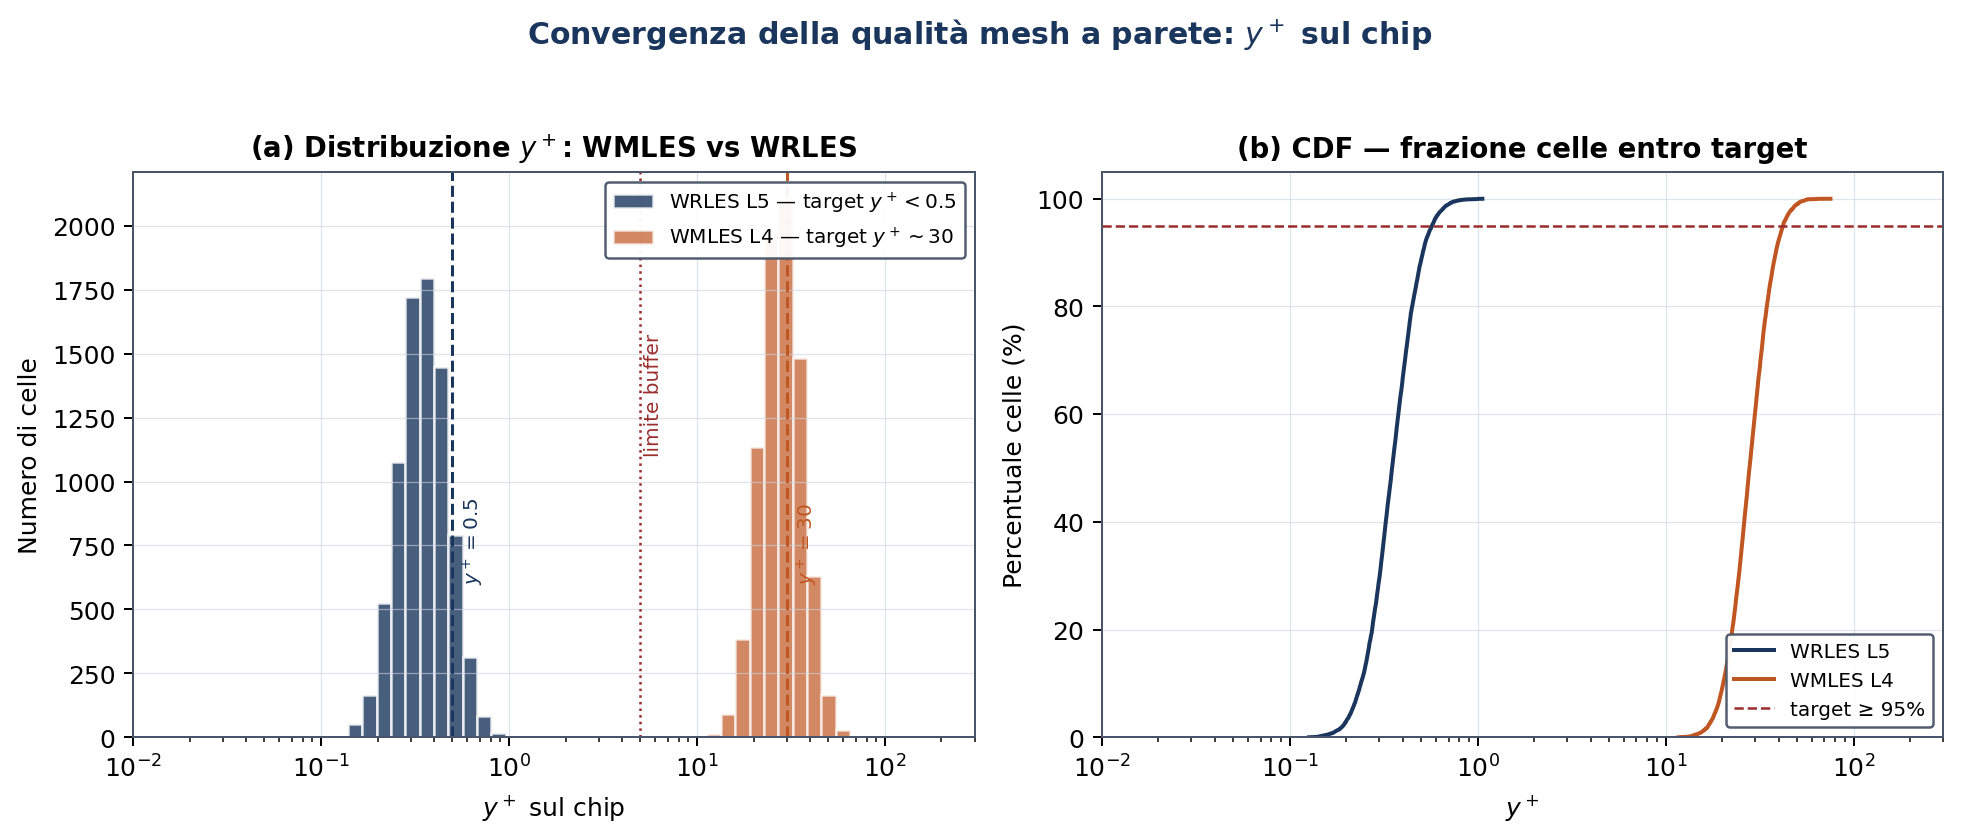
\includegraphics[width=\textwidth]{fig_yplus_histogram}
  \caption{Distribuzione del $y^+$ sulla parete del chip. (a)
    Istogrammi per WMLES L4 (arancio, target $y^+\sim 30$) e WRLES
    L5 (blu, target $y^+ < 0.5$). (b) Curve cumulative: la WRLES L5
    ha il 95\% delle celle sotto $y^+ = 1$, soddisfacendo il
    criterio.}
  \label{fig:yplus_histogram}
\end{figure}

Il criterio di accettazione per la mesh L5 è:
\begin{itemize}
  \item $y^+_{\max} < 1$ in $\geq 95\%$ delle celle del chip.
  \item Nessuna cella con $y^+ > 5$ (zona buffer non risolta).
  \item Aspect ratio prism $\leq 100$ (per evitare problemi di
    convergenza iterativa, cfr.\ Sezione~\ref{sec:residui}).
\end{itemize}

\subsection{Calcolo a priori della prima cella}

Prima di lanciare la simulazione si stima la dimensione del primo
prism layer richiesta dal $y^+$ target. Dalla relazione di Schlichting:
\begin{equation}
  \Delta y_1 = \frac{y^+\,\nu}{u_\tau},
  \qquad u_\tau \approx U\sqrt{\frac{C_f}{2}},
  \qquad C_f \approx \frac{0.079}{\Rey^{1/4}}.
\end{equation}
Per il caso Huawei ($\Rey=1000$, $U=10$\,m/s, $\nu=1.5\times 10^{-5}$\,m\(^2\)/s):
\begin{align}
  C_f &= \frac{0.079}{1000^{1/4}} = 0.0140,\\
  u_\tau &= 10 \times \sqrt{0.0070} = 0.84\,\mathrm{m/s},\\
  \Delta y_1(y^+ = 0.5) &= \frac{0.5 \times 1.5\times 10^{-5}}{0.84}
       = 8.9\mum.
\end{align}

In Ennova si imposta quindi il primo prism layer a $\sim 9\mum$, con
\emph{growth rate} 1.15--1.25 per i layer successivi. Il numero
totale di prism layer (12 per L5) è scelto per coprire $y^+ \approx
40$ con il primo strato di tetraedri.

% ============================================================
\section{Diagnostica e Troubleshooting}
\label{sec:troubleshoot}
% ============================================================

\subsection{Workflow decisionale}

Quando una simulazione presenta problemi di convergenza, è utile
seguire un protocollo standardizzato anziché applicare modifiche
casuali. La Figura~\ref{fig:flowchart} riassume il workflow
raccomandato per il progetto Huawei.

\begin{figure}[H]
  \centering
  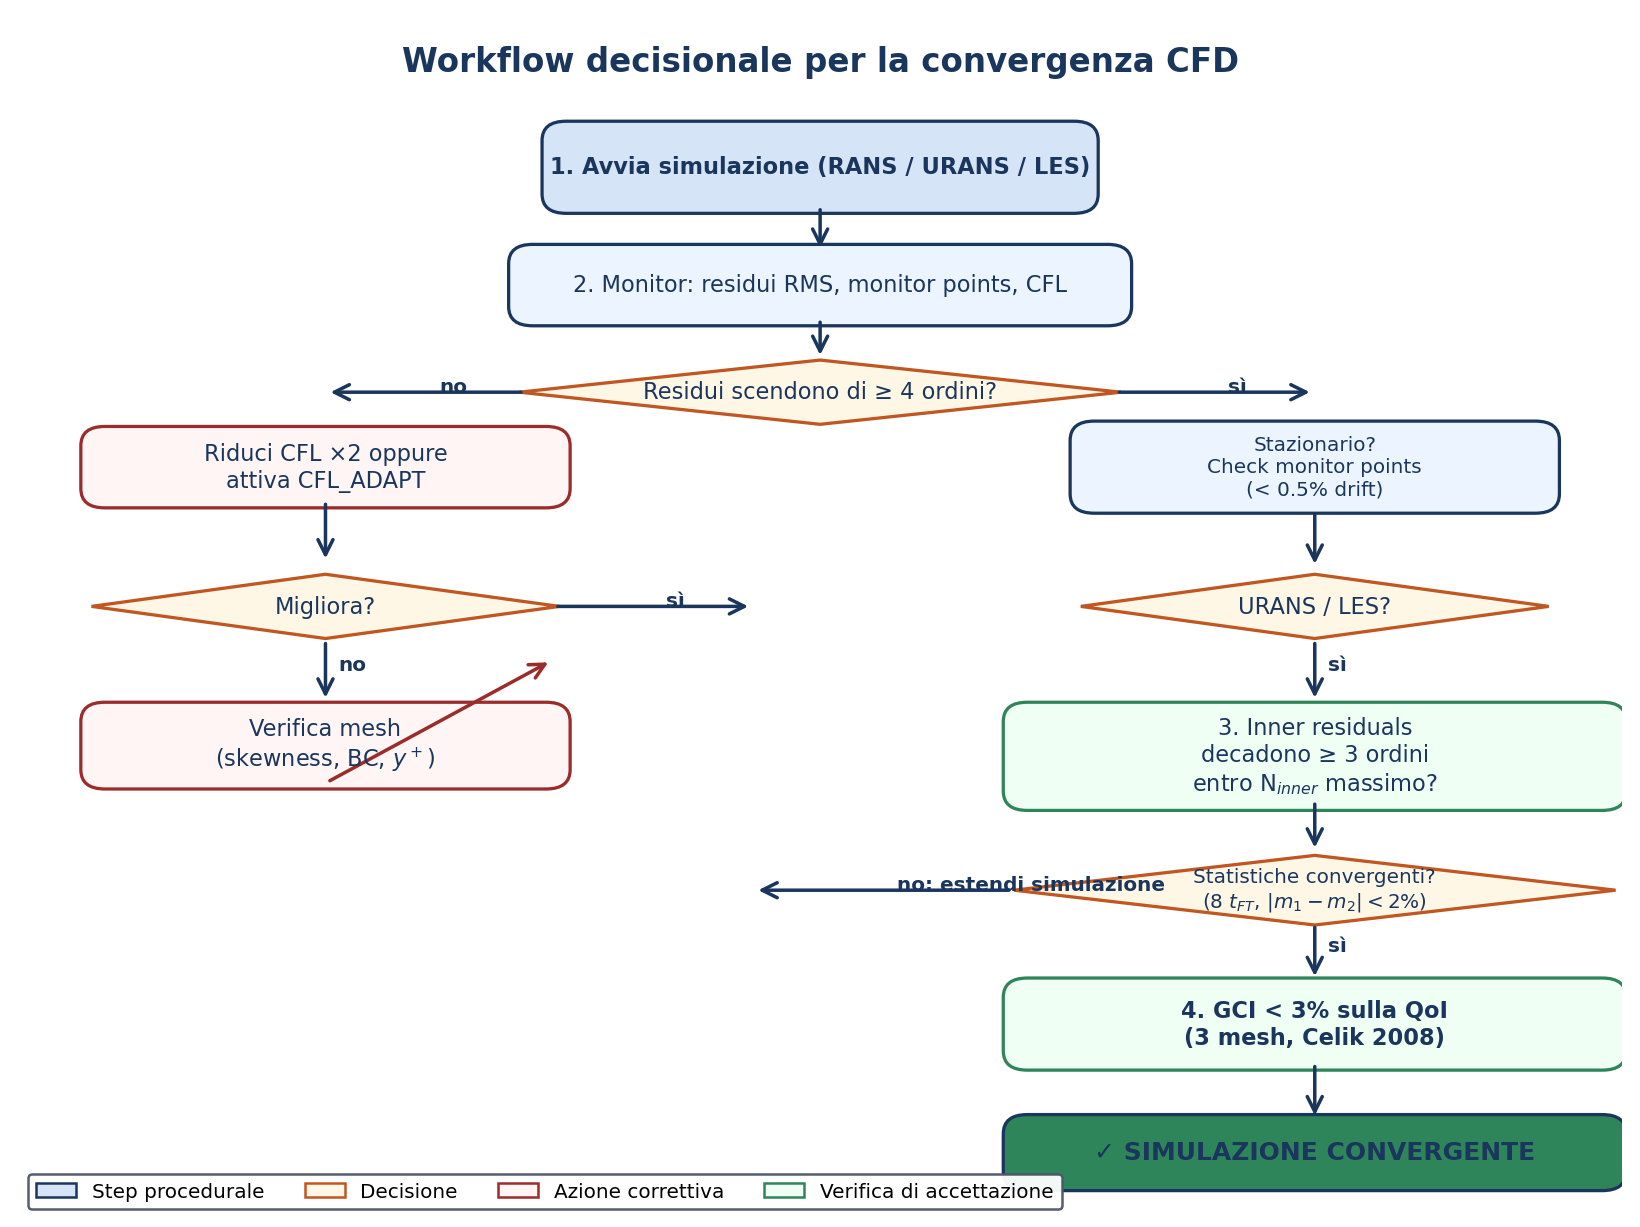
\includegraphics[width=\textwidth]{fig_flowchart}
  \caption{Workflow decisionale per la verifica della convergenza
    nelle simulazioni del caso Huawei. Il flusso parte dal monitoring
    iniziale dei residui e procede attraverso check successivi su
    convergenza iterativa, stazionarietà del campo, residui interni
    (per le simulazioni instazionarie) e GCI.}
  \label{fig:flowchart}
\end{figure}

\subsection{Tabella diagnostica: 10 sintomi e ricette}

\begin{table}[H]
  \centering
  \caption{Sintomi comuni e azioni correttive consigliate.}
  \label{tab:troubleshoot}
  \rowcolors{2}{lightblue!40}{white}
  \small
  \begin{tabularx}{\textwidth}{p{4cm}X}
    \toprule
    \rowcolor{tablehead}
    \textbf{Sintomo osservato} & \textbf{Azione consigliata} \\
    \midrule
    Divergenza esponenziale entro le prime 50 iter. &
      Ridurre \ttcfg{CFL\_NUMBER} a 0.5; verificare le condizioni
      iniziali (\ttcfg{INC\_VELOCITY\_INIT}). \\
    Divergenza dopo 200--500 iter. (cold start) &
      Attivare \ttcfg{CFL\_ADAPT= YES} con \texttt{(0.1, 1.5, 1.0, 50.0)};
      \texttt{factor\_up} più conservativo. \\
    Plateau dei residui a $10^{-2}$--$10^{-3}$ &
      Esportare il campo, individuare le celle con max residuo (in
      ParaView): tipicamente skewness, AR estremo o BC errata. \\
    Residui pressione OK ma turbolenza (\ttcfg{rms\_TKE}) bloccati &
      Verificare valori iniziali di $k$ e $\omega$; usare la formula
      di Spalart per intensità $1\%$ e scala $0.07\,\Djet$. \\
    LCO a $\sim 10^{-3}$ nei residui RANS &
      Il flusso è instazionario. Passare a URANS (\ttcfg{TIME\_DOMAIN=
      YES}, \ttcfg{TIME\_MARCHING= DUAL\_TIME\_STEPPING-2ND\_ORDER}). \\
    Inner residual non scende sotto $10^{-3}$ in 30 iter. URANS &
      Aumentare \ttcfg{INNER\_ITER} a 50; ridurre \ttcfg{TIME\_STEP}
      del 50\%; verificare $y^+$ massimo. \\
    Inner residual cresce nel tempo (per outer step successivi) &
      Possibile mesh interpolation error nella restart da L3 a L4;
      rigenerare il restart con interpolazione di secondo ordine. \\
    GCI $> 5\%$ con tre mesh L1, L2, L3 &
      Mesh non geometricamente simili o non nel range asintotico. Usare
      $r=2$ uniforme; aggiungere una mesh L4 più fine. \\
    Statistiche LES non convergono dopo $10\,\tFT$ &
      Probabile presenza di low-frequency mode; estendere a $20\,\tFT$
      o filtrare via window function (\texttt{HANN}). \\
    Spettro Welch con picchi a $f \approx \mathrm{Strouhal}\pm\mathrm{noise}$ &
      Aumentare $n_{\mathrm{perseg}}$ a $16\,384$ per migliorare
      $\Delta f$; usare segmenti con sovrapposizione $75\%$. \\
    \bottomrule
  \end{tabularx}
\end{table}

\subsection{Monitor points: il primo segnale di allarme}

Oltre ai residui RMS è raccomandato definire 4--6 \emph{monitor points}
in punti critici del dominio Huawei, salvati ad ogni step nel file
\texttt{history.dat}:

\begin{lstlisting}
% =================== MONITOR POINTS ===================
% Probe 1: stagnation point sul chip (centro del jet)
PROBE_1_LOCATION= (0.0, 0.0, 0.0)

% Probe 2: lip del tubo inlet (zona di shear layer)
PROBE_2_LOCATION= (0.00075, 0.0, 0.001)

% Probe 3: ingresso outlet laterale
PROBE_3_LOCATION= (0.010, 0.0, 0.0015)

% Probe 4: parete chip a r=D_jet (zona di riattacco)
PROBE_4_LOCATION= (0.0015, 0.0, 0.0)

HISTORY_OUTPUT= (RMS_PRESSURE, PROBE_1_PRESSURE, PROBE_2_VELOCITY-X,
                 PROBE_3_PRESSURE, PROBE_4_HEAT_FLUX)
\end{lstlisting}

In RANS, la convergenza è considerata raggiunta quando \emph{tutti} i
probe stabilizzano la loro lettura entro $\pm 0.5\%$ del valore medio
sugli ultimi 100 iterati. Questo criterio è più stringente del solo
residuo RMS e cattura situazioni dove i residui sono bassi ma il
campo continua a evolvere lentamente.

% ============================================================
\section{Checklist Riassuntiva per lo Studente}
\label{sec:checklist}
% ============================================================

\subsection{Pre-simulazione}

\begin{itemize}
  \item[\textbullet] Mesh con skewness $< 0.85$, AR prism $< 100$,
    $y^+_{\max}$ stimato $< 1$ (WRLES) o $\sim 30$ (WMLES).
  \item[\textbullet] Almeno 3 mesh disponibili (L1, L2, L3) con
    $r \approx 2$ per il GCI.
  \item[\textbullet] Condizioni al contorno coerenti
    (\ttcfg{MARKER\_INLET} velocità + \ttcfg{MARKER\_OUTLET} pressione,
    non viceversa).
  \item[\textbullet] Stima a priori del $\Delta t$ (vincolo dominante
    Kolmogorov per WRLES, CFL convettivo per WMLES).
\end{itemize}

\subsection{Durante la simulazione (RANS)}

\begin{itemize}
  \item[\textbullet] Residui RMS pressione e velocità in scala log
    monotonicamente decrescenti.
  \item[\textbullet] CFL adattivo attivo, in fase di crescita verso
    \texttt{CFL\_max}.
  \item[\textbullet] Monitor points stabili entro $\pm 0.5\%$.
  \item[\textbullet] Target raggiunto: \ttcfg{CONV\_RESIDUAL\_MINVAL=
    -6} e/o \ttcfg{CONV\_CAUCHY\_EPS} soddisfatto.
\end{itemize}

\subsection{Durante la simulazione (URANS / DDES / LES)}

\begin{itemize}
  \item[\textbullet] Inner residual scende di $\geq 3$ ordini in
    \ttcfg{INNER\_ITER} iterazioni.
  \item[\textbullet] CFL effettivo coerente con il livello di fedeltà
    ($\le 0.5$ per WRLES, $\sim 1$--$3$ per DDES/WMLES).
  \item[\textbullet] Preflush di $\geq 2.5\,\tFT$ scartato prima della
    raccolta statistiche.
  \item[\textbullet] Test del semi-intervallo: $\delta < 2\%$ sulla
    velocità media, $< 5\%$ sulla varianza.
\end{itemize}

\subsection{Post-simulazione}

\begin{itemize}
  \item[\textbullet] GCI calcolato sulla QoI principale: target
    $< 3\%$ sulla mesh fine.
  \item[\textbullet] Pope M-index $> 0.80$ in $\geq 90\%$ del volume
    (per LES).
  \item[\textbullet] Spettro Welch con $\Delta f \leq 50$\,Hz e
    $N_{\mathrm{seg}} \geq 8$.
  \item[\textbullet] $y^+$ effettivo verificato sulla soluzione
    convergente, non solo sul valore stimato a priori.
  \item[\textbullet] Confronto qualitativo dei profili medi con dati
    sperimentali Huawei (PIV, hot-wire) o con DNS di riferimento di
    Dairay et al.\ \cite{Dairay2015}.
\end{itemize}

% ============================================================
\section{Riepilogo dei Criteri Numerici per il Caso Huawei}
\label{sec:summary}
% ============================================================

La Tabella~\ref{tab:summary} sintetizza tutti i criteri numerici
discussi nel documento, organizzati per fase della pipeline.

\begin{longtable}{p{2.0cm}p{4.0cm}p{2.5cm}p{4.5cm}}
  \caption{Criteri di convergenza per fase nella pipeline Huawei.}
  \label{tab:summary} \\
  \toprule
  \rowcolor{tablehead}
  \textbf{Fase} & \textbf{Criterio} & \textbf{Soglia} &
    \textbf{Note} \\
  \midrule
  \endfirsthead
  \toprule
  \rowcolor{tablehead}
  \textbf{Fase} & \textbf{Criterio} & \textbf{Soglia} &
    \textbf{Note} \\
  \midrule
  \endhead
  \bottomrule
  \endfoot
  RANS L1 & RMS pressione & $-4$ & Debug topologia BC \\
  RANS L2 & RMS pressione + Cauchy $C_p$ & $-6$ + $10^{-6}$ &
    Mesh GCI medium \\
  RANS L3 & RMS pressione + Cauchy $C_p$ & $-6$ + $10^{-6}$ &
    Mesh GCI fine \\
  GCI & GCI$_{\mathrm{fine}}$ su $\bar u_z$ & $< 3\%$ &
    3 mesh, $r=2$, Celik 2008 \\
  $y^+$ chip & frazione celle con $y^+<1$ & $\geq 95\%$ &
    WRLES L5 \\
  URANS L2 & inner residual / outer step & $-5$ in 30 iter. &
    \texttt{INNER\_ITER}=30 \\
  DDES L3 & inner residual / outer step & $-5$ in 25 iter. &
    \texttt{INNER\_ITER}=25 \\
  WMLES L4 & inner residual / outer step & $-4$ in 20 iter. &
    \texttt{INNER\_ITER}=20 \\
  WRLES L5 & inner residual / outer step & $-4$ in 20 iter. &
    \texttt{INNER\_ITER}=20 \\
  $\Delta t$ WRLES & $\Delta t / \tau_\eta$ & $\le 0.15$ &
    $\Delta t = 0.5\mus$ \\
  Preflush LES & durata & $\ge 2.5\,\tFT$ & $= 10\ms$ \\
  Stationarity & $|\bar u_{1\mathrm{st}}-\bar u_{2\mathrm{nd}}|/\bar u$ &
    $< 2\%$ & semi-intervalli \\
  Welch $\Delta f$ & risoluzione spettrale & $\le 50$\,Hz &
    $n_{\mathrm{perseg}}=8\,192$ \\
  Welch $N_{\mathrm{seg}}$ & numero segmenti & $\ge 8$ &
    finestra Hann, overlap $50\%$ \\
  Pope M & frazione volume con $M\geq 0.80$ & $\geq 90\%$ &
    LES, criterio di Pope \\
\end{longtable}

% ============================================================
\section{Conclusioni}
\label{sec:conclusioni}
% ============================================================

Questo documento ha presentato in chiave didattica i criteri di
convergenza necessari per la conduzione affidabile della simulazione
CFD del getto impingente sul chip Huawei. I punti chiave per lo
studente sono:

\begin{enumerate}
  \item \textbf{Convergenza non è un concetto unico.} Distinguere
    sempre fra convergenza iterativa, di griglia, temporale e
    statistica. Ognuna ha indicatori, soglie e ricette correttive
    proprie.

  \item \textbf{Leggere i residui in scala log come una storia.} La
    pendenza, i plateau, le oscillazioni e le impennate sono segnali
    diagnostici precisi. La Figura~\ref{fig:residual_history} è
    materiale di riferimento da consultare per i primi mesi di lavoro
    con SU2.

  \item \textbf{Il CFL adattivo è quasi sempre la scelta migliore} per
    la fase RANS. Per le LES il CFL ha invece un ruolo di
    \emph{accuratezza}, non di velocità di convergenza.

  \item \textbf{Il GCI è non negoziabile.} Nessun risultato CFD
    industriale è credibile senza una verifica di indipendenza dalla
    griglia. Tre mesh, calcolate fino a $-6$ in residuo,
    geometricamente simili. Il caso Huawei adotta L1, L2, L3 con
    $r=2$.

  \item \textbf{Le LES richiedono pazienza statistica.} La regola
    d'oro $T \geq 8\,\tFT$ è il prezzo da pagare per medie attendibili.
    Il preflush serve a evitare di contaminare le statistiche con il
    transitorio di interpolazione tra mesh.

  \item \textbf{Il workflow decisionale} (Figura~\ref{fig:flowchart})
    e la tabella diagnostica (Tabella~\ref{tab:troubleshoot}) sono
    strumenti pratici da tenere accanto al monitor durante le
    simulazioni.
\end{enumerate}

\medskip

L'obiettivo di questo documento è duplice: da un lato costituire un
riferimento operativo per Sebastiano e collaboratori durante l'esecuzione
della commessa Huawei; dall'altro fornire allo studente che si avvicina
per la prima volta a SU2 (o a un solver CFD analogo) un manuale di
riferimento che integri le scelte fatte nel main paper con la loro
giustificazione metodologica.

% ============================================================
% RIFERIMENTI
% ============================================================
\newpage
\begin{thebibliography}{99}
\small

\bibitem{Pope2000}
  Pope, S.B. (2000).
  \textit{Turbulent Flows}.
  Cambridge University Press.

\bibitem{Celik2008}
  Celik, I.B., Ghia, U., Roache, P.J., Freitas, C.J., Coleman, H., Raad, P.E. (2008).
  Procedure for Estimation and Reporting of Uncertainty Due to Discretization in CFD Applications.
  \textit{Journal of Fluids Engineering}, 130(7), 078001.

\bibitem{Roache1997}
  Roache, P.J. (1997).
  Quantification of Uncertainty in Computational Fluid Dynamics.
  \textit{Annual Review of Fluid Mechanics}, 29, 123--160.

\bibitem{Richardson1910}
  Richardson, L.F. (1910).
  The Approximate Arithmetical Solution by Finite Differences of
  Physical Problems Involving Differential Equations.
  \textit{Philosophical Transactions of the Royal Society of London A},
  210, 307--357.

\bibitem{Welch1967}
  Welch, P.D. (1967).
  The Use of Fast Fourier Transform for the Estimation of Power
  Spectra: A Method Based on Time Averaging Over Short, Modified
  Periodograms.
  \textit{IEEE Transactions on Audio and Electroacoustics},
  15(2), 70--73.

\bibitem{Spalart2006}
  Spalart, P.R., Deck, S., Shur, M.L., Squires, K.D., Strelets, M.Kh. \& Travin, A. (2006).
  A new version of detached-eddy simulation, resistant to ambiguous grid densities.
  \textit{Theoretical and Computational Fluid Dynamics}, 20(3), 181--195.

\bibitem{Nicoud1999}
  Nicoud, F. \& Ducros, F. (1999).
  Subgrid-scale stress modelling based on the square of the velocity gradient tensor.
  \textit{Flow, Turbulence and Combustion}, 62(3), 183--200.

\bibitem{Hadziabdic2008}
  Hadziabdic, M. \& Hanjalic, K. (2008).
  Vortical structures and heat transfer in a round impinging jet.
  \textit{Journal of Fluid Mechanics}, 596, 221--260.

\bibitem{Dairay2015}
  Dairay, T., Fortune, V., Lamballais, E. \& Brizzi, L.-E. (2015).
  Direct numerical simulation of a turbulent jet impinging on a heated wall.
  \textit{Journal of Fluid Mechanics}, 764, 362--394.

\bibitem{Economon2016}
  Economon, T.D., Palacios, F., Copeland, S.R., Lukaczyk, T.W. \& Alonso, J.J. (2016).
  SU2: An Open-Source Suite for Multiphysics Design and Analysis.
  \textit{AIAA Journal}, 54(3), 828--846.

\bibitem{FfowcsHawkings1969}
  Ffowcs-Williams, J.E. \& Hawkings, D.L. (1969).
  Sound generation by turbulence and surfaces in arbitrary motion.
  \textit{Philosophical Transactions of the Royal Society of London A},
  264(1151), 321--342.

\bibitem{CFL1928}
  Courant, R., Friedrichs, K. \& Lewy, H. (1928).
  Über die partiellen Differenzengleichungen der mathematischen Physik.
  \textit{Mathematische Annalen}, 100(1), 32--74.

\end{thebibliography}

\end{document}
